%% Built on the version 1.0
% Version 1.3 after reviewer comments
% Version 1.2 after submission to conference and comments from co-authors.
%Version 1.1 CAT Added self protection simulations.
%Version 1.0 CAT

\documentclass[english, 12pt]{report}
\PassOptionsToPackage{hyphens}{url}\usepackage[colorlinks,hyperfootnotes=false]{hyperref}
\hypersetup{pdffitwindow=true,linkcolor=black,citecolor=black,urlcolor=black,menucolor=black} 
\usepackage{mathptmx}
\usepackage[T1]{fontenc}
\usepackage[latin1]{inputenc}
\usepackage[a4paper,margin=2cm,headheight=10mm,headsep=12mm,footskip=12mm,bmargin=27mm,tmargin=32mm]{geometry}
\usepackage{graphicx}
\usepackage{fancyhdr}
\pagestyle{fancy}
\setlength{\parskip}{\medskipamount}
\setlength{\parindent}{0pt}
\usepackage{array}
\usepackage{float}
\usepackage{setspace}
\usepackage{tabu}
\usepackage{amsmath}
\usepackage{easy-todo}
\usepackage[caption=false]{subfig}
\onehalfspacing
%\usepackage{showframe}

\makeatletter

%%%%%%%%%%%%%%%%%%%%%%%%%%%%%% LyX specific LaTeX commands.
\providecommand{\LyX}{L\kern-.1667em\lower.25em\hbox{Y}\kern-.125emX\@}
%% Because html converters don't know tabularnewline
\providecommand{\tabularnewline}{\\}

%%%%%%%%%%%%%%%%%%%%%%%%%%%%%% User specified LaTeX commands.

\def\docnumber{rrsg:00}
\def\docrevnum{1.1}
\def\userdate{\today}
\def\classification{Draft}
\def\docname{\jobname}

% Define PostScript graphics command
\special{header=figs/rrsglogo.h}

% Save graphics in LaTeX box
\newsavebox{\rrsglogo}
\sbox{\rrsglogo}{
\includegraphics[totalheight=10mm]{figs/rrsglogo.pdf}}

% Header and Footer Line Widths
\renewcommand{\headrulewidth}{0.4pt}
\renewcommand{\footrulewidth}{0.4pt}
\flushbottom

\fancyhead{}                 % Clear all header fields

\fancyhead[L]
{
{ \em UCT Radar Remote \\ Sensing Group}
}

\fancyhead[C]{\usebox{\rrsglogo}}

\fancyhead[R]
{
{ \em Department of ~ \\ 
  Electrical Engineering}
}

\fancyfoot{}                   % Clear all footer fields

\fancyfoot[L]
{
{ Document No.~\docnumber \\ 
  Document Rev.~\docrevnum}
}

\fancyfoot[C]
{
{~\\ \classification}
}

\fancyfoot[R]
{
{ \userdate ~~ \\ 
  Page:  \thepage~of~\pageref{lastpg}}
}

\makeatother

\usepackage{babel}
\begin{document}

\title{\vspace{1in}A Study of Commensal Radar in terms of Electronic Defence (ECM, ECCM)}


\author{M. Inggs, D. W. O'Hagan, C. Tong}


\date{\userdate\\
\vspace{1in}File: \docname\\
Document No: \docnumber}

\maketitle
\newpage


\begin{table}[H]
\begin{centering}
\textbf{\large Approval}
\par\end{centering}{\large \par}

\centering{}%
\begin{tabular}{|m{23mm}|m{20mm}|m{25mm}|m{33mm}|m{19mm}|m{23mm}|}
\hline 
 & \centering{}\emph{Name} & \centering{}\emph{Designation} & \centering{}\emph{Affiliation} & \centering{}\emph{Date} & \centering{}\emph{Signature}\tabularnewline
\hline 
\hline 
Submitted by &  &  &  &  & \tabularnewline
\hline 
Reviewed by &  &  &  &  & \tabularnewline
\hline 
Accepted by &  &  &  &  & \tabularnewline
\hline 
Approved by &  &  &  &  & \tabularnewline
\hline 
Approved by &  &  &  &  & \tabularnewline
\hline 
Approved by &  &  &  &  & \tabularnewline
\hline 
\end{tabular}
\end{table}


\begin{table}[H]
\begin{centering}
\textbf{\large Document History}
\par\end{centering}{\large \par}

\centering{}%
\begin{tabular}{|>{\centering}m{20mm}|>{\centering}m{30mm}|>{\centering}m{25mm}|m{84mm}|}
\hline 
\centering{}\emph{Revision} & \centering{}\emph{Date of Issue} & \centering{}\emph{RRSG Number} & \centering{}\emph{Comments}\tabularnewline
\hline 
\hline 
0& April 2015 & NA & Working draft. \tabularnewline
\hline 
1.0 & 22-04-14  & NA & Draft for Thun presentations \tabularnewline
\hline 

\docrevnum & \userdate & \docnumber & What is special about this version? Short summary of key change(s)\tabularnewline
\hline 
 \end{tabular}
\end{table}


\begin{table}[H]
\begin{centering}
\textbf{\large Document Software}
\par\end{centering}{\large \par}

\centering{}%
\begin{tabular}{|m{35mm}|>{\centering}m{35mm}|>{\centering}m{20mm}|>{\centering}m{62mm}|}
\hline 
 Text Processor& \centering{}\emph{Package} & \centering{}\emph{Version} & \centering{}\emph{Filename}\tabularnewline
\hline 
\hline 
& TeXShop & 3.5 & \docname \tabularnewline
\hline 
 &  &  & \tabularnewline
\hline 
 &  &  & \tabularnewline
\hline 
\end{tabular}
\end{table}


\begin{table}[H]
\begin{centering}
\textbf{\large Company Details}
\par\end{centering}{\large \par}

\centering{}%
\begin{tabular}{|m{30mm}|m{130mm}|}
\hline 
Name & Radar Remote Sensing Group, University of Cape Town\tabularnewline
\hline 
Physical Address & Department of Electrical Engineering, George Menzies Room 7.16, University
of Cape Town, Upper Campus, Rondebosch \tabularnewline
\hline 
Postal Address & Department of Electrical Engineering, George Menzies Room 7.16, University
of Cape Town, Private Bag, Rondebosch 7701, South Africa\tabularnewline
\hline 
Telephone & +27 (0)21 650 2799\tabularnewline
\hline 
Fax & +27 (0)21 650 3465\tabularnewline
\hline 
Email & mikings@gmail.com\tabularnewline
\hline 
\end{tabular}
\end{table}


\newpage

\tableofcontents{}

\newpage

\listoffigures


\newpage

\listoftables


\newpage

% Comment out for document production.
\listoftodos


%=========================
\chapter{Scope}


\section{Identification}

This is a study.


\section{Purpose}

This document describes the scope of a study to be carried out for armasuisse, detailing the operation of Commensal Radar in terms of ECM against Commensal Radar and ECCM that can be deployed in mitigation of the ECM.

%
\section{Introduction}


In this document we study the major topics of the susceptibility of Commensal\footnote{The origin of the term Commensal is discussed in Chapter 2} Radar (CR) to countermeasures (ECM) (jamming and possible deception) and then,  possible counter-countermeasures (ECCM) by the CR system against a malicious entity. We first outline the User's Requirements for this study, which are given verbatim in an appendix to this document, and has provided the major guidance to work reported.

We note that the scope of the study is limited in terms of funding (hence time), and we have taken the approach of wider coverage, at the expense of depth in some places, and will indicate the direction of further work.

The report begins with an overview of the basic operation of CR and then presents a taxonomy for \emph{unconventional radars} that classifies according to their use of transmitters and their architecture. We do this because the naming conventions in current use are not uniform, and sometimes obscure, or misleading. No radar system can be \emph{passive}, and thus the term, \emph{passive}, while accepted, is incorrect. Furthermore, the term precludes situations where the transmitter might be collaborative i.e. the radar and other system (often a communications system) have a \emph{symbiotic} relationship. We refer to systems that use transmitters of opportunity, without any form of collaboration as, \emph{commensal}. This overview also discusses the processing used for CR.

We follow with a review of the very limited publications in the area of the jamming of CR systems, ECM and ECCM. This is given in the form of a list of references and short overviews. However, the material found in the review influences the following three sections, and we indicate where the discussion is taken up further. We also speculate on topics that are not discussed in the open literature. 

The next chapter considers methods for jamming a Commensal Radar (i.e. simple denial of service). These activities  will require Electronic Support Measures (ESM) to be effective, as well as strong intelligence inputs about physical infrastructure. We discuss the effectiveness of common jamming methods to disturb passive radars, under the assumption that receiver sites are known / unknown. What are the distinctions between single frequency networks (e.g. DAB, DVB) and FM broadcast in terms of susceptibility to jamming. We discuss which waveforms are appropriate for jamming (broadband, noise, specific waveforms\ldots). We mention that when considering the power and bandwidth of jamming emitters that the possibility that the CR under attack might use the jammer as a transmitter of opportunity ECCM). We conclude this chapter by looking at spot and barrage (noise) jamming.

The discussion  then moves onto more subtle techniques such as deception ECM (DECM). Approaches that might deceive a CR system are conceived. Is it possible to deceive a CR system to give an indication of wrong targets or wrong target positions?  A big consideration here is that it will be difficult due to the multistatic geometry (multiple angle illumination of targets). What is the effectiveness of the interfering transmitter that emits the original broadcast signals with time delays and / or Doppler shifts (repeater techniques, DRFM jamming)?

The CR system can deploy ECCM to protect itself. There are a large number of possibilities, exploiting signal processing, beam steering and spatial diversity. In a short report, we can only give some suggestions. However, we show through simulation the effectiveness of null steering.

 The report concludes with a summary, indicating where further work is required. As mentioned earlier in this section, this report is scoped to present the possibilities for defeating CR systems, rather than providing detailed analysis of all cases. The possibilities are huge, due to the diverse nature of CR systems, compounded with the geometries.


%================================
\chapter{Commensal Radar Fundamentals and Taxonomy}
%================================

The report begins with an overview of the basic operation of CR and then presents a taxonomy for unconventional radars that classifies according to their use of transmitters and their architecture. We do this is because the naming conventions in current use are not uniform, and sometimes obscure. No radar system can be passive, and thus the term, ``passive'' while accepted, is incorrect. Furthermore, the term precludes situations where a transmitter might be provided for a system that is normally dependent on transmitters of opportunity, or, collaborative.
%_____________________________
\section{Taxonomy for EM Sensors}


Based on at least an introductory level knowledge of Radar, and unconventional radar, with receive only sensing (Commensal Radar) we now introduce a more logical taxonomy that can be applied to all electromagnetic sensors. We will not dwell on, for example, optical sensors, and focus on the ``receive only'' systems, currently known as, ``passive radar''.

\begin{figure}[htbp]
\begin{center}
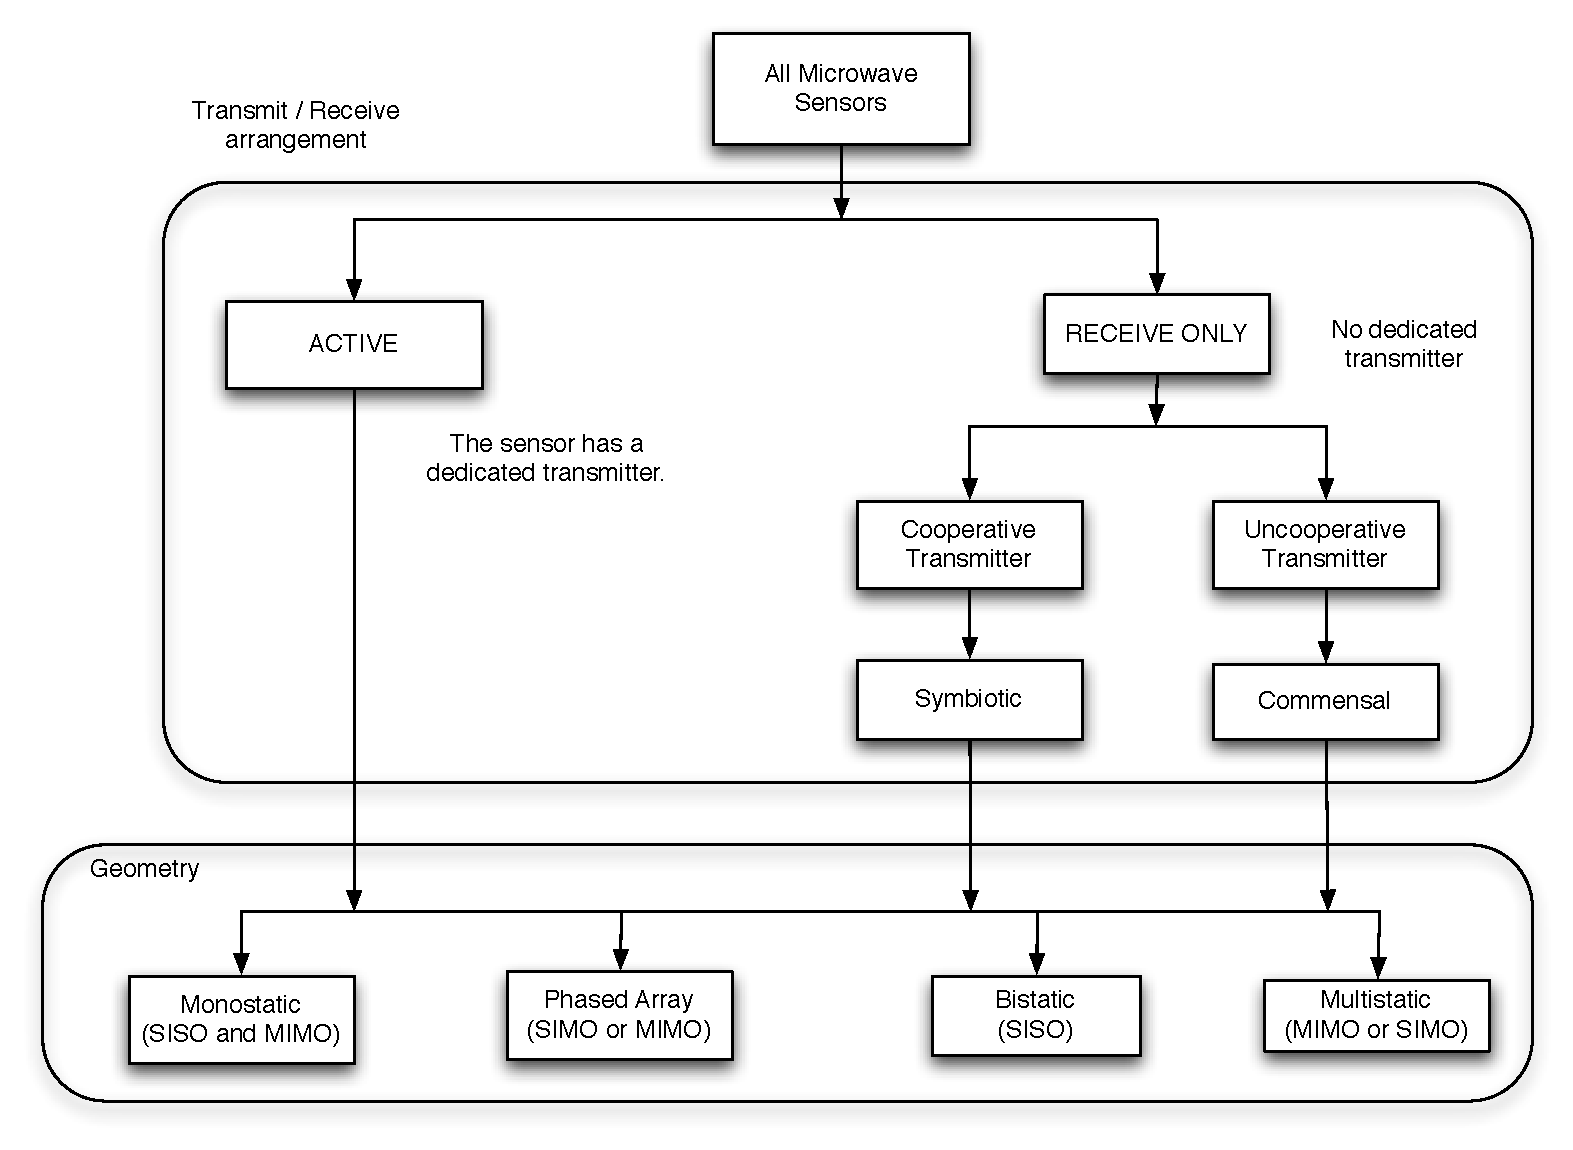
\includegraphics[width=\textwidth, angle=90]{figs/tree_4}
\caption{A taxonomy for all EM sensors.}
\label{fig:tax}
\end{center}
\end{figure}


Referring to the figure~\ref{fig:tax} we have split EM sensors into two branches i.e. those that have a transmitter as an integral part of their design, and those without (presently known as, ``passive''). We do not discuss the left hand branch further.

The ``passive'' branch is split into two i.e. but share the property that the transmitter is not part of the system i.e. the transmitter is integrated into another system. Using terms common in Biology and Natural Sciences, the left branch is termed, ``symbiotic'' and the right hand one, ``commensal''. The transmitter of a ``symbiotic'' system is differentiated from the ``commensal branch'' in that the former is designed to provide signals suitable for the radar function of the ``symbiotic'' radar system. An example is the proposed ``White Space Symbiotic Radar''~\cite{inggs:14j} that operates in the White Space Frequency Band (600 - 800 MHz). The primary function of the system is a network of sensors conforming to IEEE~802.22 providing a sparse network for internet provisioning. However, the ``White Space Symbiotic Radar'' system has influenced the design of the communications waveforms utilised to ensure their suitability for radar (range resolution, Doppler resolution, for example). 

The Commensal branch, however, uses transmitters of opportunity. They have no influence on the waveforms, frequency of operation, or, position of the transmitters. Examples of this are numerous e.g. FM Broadcast ~\cite{ohagan1}, DVB ~\cite{kuschel4}, etc.

The figure delivers all the different type of radar to a common block, labelled, ``MIMO''. ``MIMO'' (Multiple Input, Multiple Output) is a concept from communications, that describes a communications system that uses a number of transmitters (or waveforms in a single transmitter) to communicate to a receiver system that has a number of spatially distributed receivers. The received signals are combined to provide a better signal to noise ratio. Clearly we can consider a degenerate case of 1:1 MIMO, which can describe a monostatic radar (same site for transmitter and receiver), or, a bistatic radar, where the transmitter is separate from the receiver. The variety of channel combinations is huge, with waveform and spatial diversity being exploited in ingenious ways.

This study discusses the most common form of ``passive'' (actually, ``receive only'') in the Commensal Radar (CR) format i.e. no influence on the transmitter carrier frequency, waveform, or position. Common examples are the use of FM Broadcast and DVB transmissions.

\section{Current Interest in CR}

Comment from a report by Arend G Westra~\cite{westra:09} 

\begin{quote}The USA should] Endeavor to be a leader in the passive
radar field. Arguably, the United States has
marginalized the passive radar field due to
a focus on conventional radar systems. The
U.S. military must gain an understanding
of passive radar, not merely theoretically, or
with minor research and development projects,
but with a dedicated effort. But why, one
may ask, build a stealth counter when there
is no immediate stealth peer competitor? The
answer is that would-be competitors in the
stealth arena are making a dedicated push to
develop this technology. We cannot afford to
spend billions on stealth, only to fail to thoroughly
understand and counter rival systems.
\end{quote}

Another example promoting the future of CR is from Griffiths et al.~\cite{griffiths1}

\begin{quote}The principal advantages
of bistatic radar are (i) the fact that the receiver is passive,
making it far less vulnerable to electronic counter measures
(ECM) and (ii) it is a counter to stealth technology, which
is designed primarily to defeat monostatic radar. In
addition multiple receivers can be employed, each one
forming a bistatic radar with the single transmitter. This
offers the potential for tailored coverage and a richer
information source to enable more accurate location, high
resolution imaging and target reconstruction. The price to
be paid for these advantages is an increase in system
complexity and processing.
\end{quote}

However, nothing is said about the specific advantages of CR in the ECM environment, and, as we shall see, this is not a simple matter.

\section{Commensal Radar Basics}

The report is prefaced with the fact that the audience will have attended the one day course given by Assoc Prof. Daniel W. O'Hagan on the 20th April. The material presented here is an overview of the operation of Commensal Radar, including a brief view of the signal processing. Based on the introduction,  we then introduce a level of sophistication in the form of a Taxonomy that applies to all EM sensors.

%<<<<<<<<<<<<<<<<<<<<<<<<<<<<<<<<<<<<<<
% Background on ECM from Daniel
\section{Short Overview of Bistatic and CR}

For a thorough reading on the theory of bistatic and CR, \cite{willis}, \cite{willis1}, \cite{chern} and \cite{chern1}, represent comprehensive texts. Furthermore, the tutorial given on Monday 21st April to armasuisse by Daniel O'Hagan, also covers most of the essential theory. 

\begin{figure}[]
\centering
  % Requires graphicx.sty
  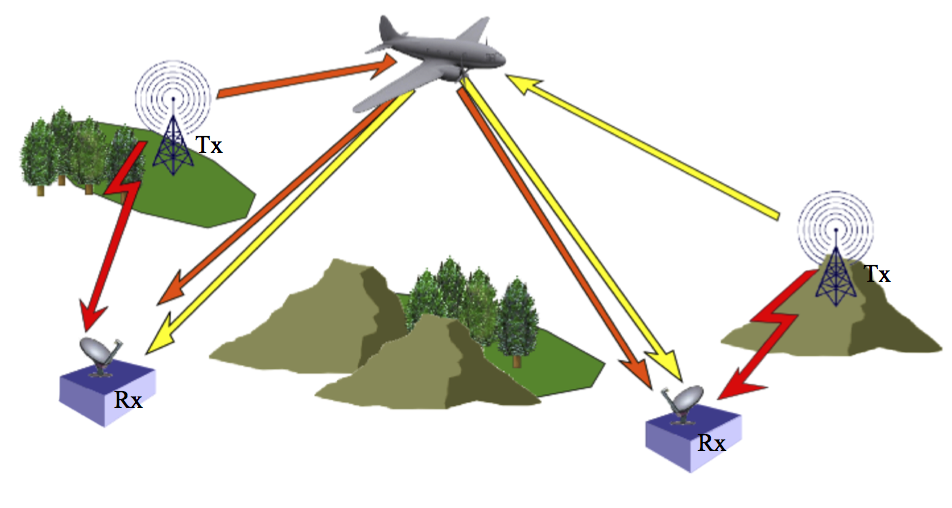
\includegraphics{./figs/CR_1}
  \caption{Depicting a Multistatic Radar}\label{fig:CR_1}
\end{figure}


A bistatic radar uses antennas for transmission and reception at sufficiently different locations that the angles or ranges to the target are significantly different \cite{stand}.

A Commensal Radar (CR) relies on pre-existing transmitter infrastructure to illuminate the target while the receiver receives the scattered energy. These illuminators of opportunity are usually non-cooperative transmitters such as:

\begin{itemize}
\item FM radio
\item DAB 
\item DVB 
\item GSM 
\item Satellite 
\end{itemize}


Some top-level characteristic of CR are listed: 

\begin{itemize}
\item Commensal radars do not need RF spectrum allocation
\item Discovery of the CR receiver is difficult
\item High resistance to Electronic Countermeasures
\item Spatial and frequency diversity possible
\item Possible enhanced RCS at some geometries,
\item Forward Scatter
\item Illumination tilted-downwards for better for low-altitude surveillance
\item Depending on illuminator, range resolution can be fine (DVB) or coarse (FM)
\item Detection capabilities not well defined
\item CR Rx can be made mobile and rapidly deployable to conform to tactics such as frequent sensor relocation to deny enemy fixed targeting
\item CRs easier to replace than expensive air-defence systems


\end{itemize}


\section{CR Literature Review}

This review provides an overview of some important literature relating to CR. In recent years there has been a huge increase in CR-related publications in journals and conferences. The majority of recent publications pertain to algorithmic refinements of CR processing. 

Whilst the amount of CR-related publications has grown in recent years, there are very few publications in the open literature that focus on ECM applied to CR. Internet searches yield hits that mention various research programmes and suggestions for ECM against CR, however, there is little material that is of a technical rigour requiring review.

The NATO group SET-164 (led by Daniel W. O'Hagan) has produced a comprehensive report on CR performance, particularly with regards to clutter modelling. The SET-164 report has been approved for release to Switzerland in 2014.

At least one NATO group, SCI-190 \textit{Electronic Countermeasures to Radar with High-Resolution and Extended Coherent Processing}, has studied countermeasure against CR. SCI-190 was not exclusively focused on ECM against CR, but it formed part of their remit. The SCI-190 group comprised ECM experts from Europe and the US. The group was led Dietmar Mattes of Fraunhofer FHR. The present author attended one SCI-190 meetings and delivered a briefing on CR. The informal consensus amongst the SCI-190 grouping was that ECM applied to CR is ``not easy''.

The review for this report provides an overview of some influential bistatic radar experiments using illuminators of opportunity.  Beginning with a brief discussion of potential illuminators, and the criteria that each should satisfy before being considered 'desirable' for a particular application, there follows a more in-depth assessment of experiments involving these illuminators.  

There are numerous illuminators of opportunity that can potentially be utilised, with some having more desirable radar characteristics than others.  They include: HF radio signals, VHF FM radio signals, DAB, DVB, GSM, GPS, and satellite broadcast services.  There are several conditions that must be satisfied before an illuminator can be considered 'desirable': (i) The transmit power must be sufficient for the coverage required.  (ii) There should be accord between the modulation bandwidth of the illuminating source and the desired range and Doppler resolution. 

The ambiguity function of the more random-like signals will approach the ideal ``thumbtack'' response. A thumbtack ambiguity response represents an excellent ability to discriminate between targets in both range and Doppler. It is important to note, however, that signals producing thumbtack ambiguity functions have a poor Doppler tolerance and are not well suited for targets that can rapidly accelerate and decelerate.  

In \cite{griffiths1986}, Griffiths and Long used analogue television broadcasts from the Crystal Palace transmitter in South London as the illuminator of opportunity to detect aircraft landing and taking off from Heathrow airport.  The receiver was situated at University College London (UCL), 11.8 km from the transmitter.  The transmitted signal was omni-directional with an ERP of 1 MW and operated on four TV channels between 487.25 and 567.25 MHz, with an individual channel bandwidth of 8 MHz, corresponding to 250 kW/channel. The autocorrelation function of the sync-plus-white waveform inherent to analogue television produced high range sidelobes in the order of 5 dB which obscured targets.  It also provided poor range resolution and severe ambiguities at 9600 m and at multiples thereof.  Griffiths and Long concluded that the analogue television signal was not an ideal illuminator of opportunity since its autocorrelation function exhibited broad peaks at 64 $\mu$s intervals corresponding to the line sync pulses.  

In a later work \cite{howland1999} Howland managed to extract Doppler and bearing information from the echoes of the analogue television video carrier to detect and track aircraft at ranges of up to 260 km.  In this application Howland was not concerned with the modulation of the signal and hence did not experience the ambiguities outlined in \cite{griffiths1986}.  Howland's processing exploited the fact that it is possible to achieve a very accurate measure of target Doppler shift using a stable carrier frequency.  Howland, like Griffiths, had a dual channel receiver, one for the reference and the other for target surveillance.  The baseline distance between the Crystal Palace transmitter and the receiver at Pershore was 150 km.  He constructed a phase interferometer consisting of a pair of Yagi antennas separated by 0.6$\lambda$.  It was found that the mutual coupling between the antennas caused inaccuracies in the bearing measurements and had to be compensated for.  As the receiver was situated beyond the Line-of-Sight (LoS) of the transmitter, the direct path interference was substantially reduced.  Howland reported that aircraft could be tracked to ranges up to 260 km from the receiver and 100 km from the transmitter out into the English Channel.  

Zoeller et al. in \cite{zoeller} described a CR system that utilised commercial FM broadcasts as the illuminating signal.  FM radio signals are attractive due to their copious availability; comparatively high transmit powers, and random (noise-like) features, which mean that their ambiguity function (depending on suitable programme content) can approach the ideal thumbtack response.  Zoeller found that, due to the low carrier frequency of FM broadcasts, the CR receiver must use long processing intervals to obtain good Doppler resolution.  The processing intervals ranged from 0.125 to 0.5 seconds which equated to range-rate (velocity) resolutions from 3 m/s to 12 m/s. However, processing intervals of 1 s or more are typically reported in the literature.  Like the other techniques described, their system consisted of two channels, designated reference and target (surveillance).  Zoeller concluded that proper siting of the system is critical to system performance.  This particular system was located on top of Green Mountain, Alabama, USA and allowed detection of commercial aircraft to about 100 km.

A stage of analogue direct signal cancellation in a CR system is desirable as it places a less stringent requirement on the ADC dynamic range.  The UK BAE Systems Multiband Passive Radar Demonstrator \cite{pollard} employed an analogue canceller for this very reason.  It was designed to be configurable to suppress direct signal contributions from a number of different transmission types including DAB. 

In work reported in 2005, Howland, Maksimiuk and Reitsma \cite{howland2005}, now working for the NATO CIA (NCIA) in The Hague, developed a CR system that utilised an FM transmitter located at Lopik, approximately 50 km from the receiver.  As a result of the shorter baseline, Howland suffered a significant increase in direct signal breakthrough compared with that in his previous work described above and in \cite{howland1999}.  In an attempt at reducing the breakthrough, a null in the antenna cardioid was physically steered in the direction of the transmitter.  Once the direct signal had been adaptively filtered, the data could be processed to search for Doppler-shifted and time-delayed echoes of any targets that may be present. 

The receiver bandwidth in \cite{howland2005} was comparable to that of an individual broadcast station resulting in a range resolution of 2 - 3 km.  The authors claimed that this signal clearly offered ``useful target ranging information''.  Whilst upon initial reading this value of range resolution could be considered inadequate, it is important to note that their system detected and tracked large passenger-jet aircraft to ranges in excess of 150 km from the receiver.  As this was the case, then a range resolution of 1.5 km did indeed offer useful ranging information.

As Howland and others have experienced, the greatest single limitation to CW bistatic radar performance is the presence of the Direct Signal Interference (DSI).  O'Hagan and Colone et al in \cite{ohagan1} discussed further the issues of the DSI.  The authors estimated that the target echo can be as low as 90 dB below the DSI breakthrough.  This situation can be improved if the surveillance antenna is shielded from the DSI \cite{ohagan2}, \cite{ohagan3} and \cite{ohagan4}.

In \cite{ohagan1}, due to the positioning of the antennas, the UCL building also acted as a shield from the direct signal.  This form of physical shielding (using the UCL building) achieved a suppression of about 12 dB. 

Research has been conducted towards looking at the suitability of Global System for Mobile communication (GSM) transmissions for use in CR systems.  The advantage of these is that there are GSM base stations honeycombed across large urban areas.  Although the individual transmit power of a GSM base station is low compared to that of FM radio, typically less than 50 W and with a cell range radius less than 2 km, this may by reconciled by their abundance.  GSM transmissions occupy the 870 - 960 MHz band with linear vertical polarisation.  A single sector GMS antenna has an azimuth beamwidth of 60$^\circ$ and an elevation beamwidth of 16.5$^\circ$.  The length of the antenna sector is 1.5 m and the beam tilt can be set between $\pm$12$^\circ$.  The gain of such elements is 15 dBi \cite{kitchen}.  Tan et al. in \cite{tan} investigated the feasibility of using GSM to detect and track different types of ground moving targets, such as vehicle and human movement.  Unlike FM and analogue TV broadcast signals, where the signal changes as a function of the programme content, the effective bandwidth of a GSM carrier signal is constant.  Tan et al. report a maximum range resolution of 1.845 km with a theoretical carrier bandwidth of 81.3 kHz.  Since the small bandwidths of a GSM carrier signal (81.3 kHz) resulted in a range resolution comparable to that of a single FM channel, it was too poor to discriminate between the human and vehicle targets. However, Tan demonstrated results for the Doppler tracking of cooperative ground-moving targets (i.e. a small truck and a human).

In separate work Poullin \cite{poullin} investigated CR based on digital broadcast signals (DAB, DVB) with Coded Orthogonal Frequency Division Multiplexing (COFDM) modulation.  

It is often the case that weak target echoes at far ranges are masked by stronger echoes from closer-in targets.  This masking effect is due to the high peak-sidelobe level of the ambiguity function and cannot be removed by conventional Moving Target Indicator (MTI) techniques because of the extensive range-Doppler spreading of the interference.  The situation is well covered by Kulpa and Czekala in \cite{kulpa1} and by Colone and O'Hagan et al. in \cite{ohagan5}.  In \cite{kulpa1}, strong multipath and target echoes are progressively cancelled (whilst retaining in memory the location of the strong targets).  However in \cite{ohagan5}, a multistage processing algorithm was developed for disturbance cancellation and target detection based on projections of the received signals in a subspace orthogonal to both the disturbance and previously detected targets.  The technique dealt with the interference spreading in the Doppler dimension by processing the data in short batches and later recombining each batch. This permitted a wider cancellation notch in the Doppler domain thus yielding an improved removal of the disturbance together with a reduced computational load.  Unlike Kulpa's and Czekala's technique, the cancellation method in \cite{ohagan5} has been tested and operates well on real FM data, thus extending the detection range of the passive radar.

In around 2005, one of the very few commercially available CRs was the Lockheed Martin Silent Sentry system that utilised FM radio broadcast transmissions.  Silent Sentry could be deployed on a fixed or a mobile (vehicle) platform.  The radar use a vertically polarised circular array antenna, which was 1.5 m tall and comprised eight dipoles arranged evenly on a 1 m diameter cylinder.  The final iteration the radar had the dipoles arranged on a 2 m diameter circle for generating narrower and higher gain beams, thus providing greater range and higher accuracy.  Tests have shown that the sidelobe levels were sufficiently high that they impeded target tracking.  However, modifications to the antenna, such as the addition of parasitic elements to uniformly increase the bandwidth over the FM band and compensating for mutual coupling, were expected to achieve a PSLR of around 30 dB.  Another antenna option was available in the form of a horizontally polarised linear array of dipoles for extended range sector coverage.  The linear array was deployed for longer range applications (200 km).  Silent Sentry 3 version 2 (SS3v2) provided four times the processing capability over its earlier iteration, SS3v1.  It had ten RF input channels providing the potential for greater system flexibility for the addition of extra antennas, or for continuously monitoring the signal environment.  The latter case is particularly useful for accurately predicting the propagation conditions.  The Lockheed Martin engineers have found that they occasionally experience ducting, which is an inversion in the thermal layer that results in propagation anomalies, so a signal monitoring channel could provide intelligence about possible environmental anomalies \cite{lockheed}.

BAE Systems and Roke Manor Research created the CELLphone raDAR (CELLDAR) system. CELLDAR utilised transmission from GSM 900, 1800 and 1900 mobile phone broadcasts and operated in a multistatic radar configuration. The system was intended for the detection and tracking of moving air, land and sea-based objects \cite{celldar}.  The system suffers significantly from interference from cars, thus limiting detection performance \cite{rickett}.  To improve and enhance system performance, CELLDAR also encompassed acoustic sensors (translates the Doppler frequency into the audio band) to 'hear' emissions from the target. The present programme status of CELLDAR is not known, but it is likely that the project has ceased.

Despite the commercial failure of Silent Sentry and CELLDAR, several other organisations with long traditions in radar have CR Research and Development programmes. Some of these, including Thales, Airbus, and Selex currently offer (or are soon to offer) CR as commercial products. Thales with their Homeland Alerter (HA-100) and Airbus (formerly Cassidian) with their Passive Radar have been leading the commercial drive for CR technology.

The HA-100 is relies on FM illuminators whilst the Airbus Passive Radar employs a multiband approach encompassing FM, DAB and DVB. Both systems have developed rapidly over the past five years. Their performance improvements have been impressive with significant refinements to system hardware and signal processing. Both Thales and Airbus have developed advances Mission Planning Tools, antenna array beamforming and null-steering, robust interference suppression techniques.

Fraunhofer FHR is not a commercial enterprise but it collaborates closely with Airbus and Thales. FHR itself has focused primarily on DAB and DVB based CRs and has developed a number of demonstrator systems including DELIA (DAB), SANDY (DAB), CoRa (DAB and DVB), and CoRa-11 (11-element array DVB CR).

The German and French Ministries of Defence are enthusiastic about CR technology and are keen for CR to form part of the air-defence infrastructure.  In the civilian context, CR is also being seriously considered as a supplementary technology for Air Traffic Management (ATM).

According to \cite{caa_1}, the UK Civil Aviation Authority (CAA) strategy with regards to CR can be summarised as:

\begin{itemize}
\item Future ATM capability based on combination of independent ground-based surveillance and airborne derived down-linked data, driven by performance requirements and new technology.

\item Still be a requirement for PSR coverage by primary radar due to national defence and system security needs. Primary radar will be used as a back-up system and as a means of tracking non-cooperative users. 

\item Multi-static PSR is a replacement for the current primary radar solution that is more cost-effective and reduces spectrum requirements. Further proof of concept work is required before multi-static PSR is accepted as a primary surveillance means.

\item A CAA roadmap for implementation of changes to surveillance over the next 20 years plans the ``introduction of Multi-Static PSR to replace primary radar'' in 2015 to 2020.

\item Beyond 2020, the CAA plan a ``Wider roll out of Multi-Static PSR''.
 
\end{itemize}

The ERA Company in the Czech Republic are currently developing an Passive Emitter Tracker (PET) and CR dual operation system. Likewise, a consortium in Poland including Warsaw University of Technology, the Ministry of Defence and radar industry are also developing a PET-CR system, which is intended to be at TRL-9 upon project completion.

   % supplied by Daniel

\section{Diversity}

We note that any CR system must be diverse in terms of either frequency of operation or multiple receivers, spatially separated, or, both of the previous. We look at some examples. The combinations are enormous, so the analysis is only partial. However, the said diversity is a critically important part of a CR system's defence against countermeasures, and also provides ECCM possibilities. 

\subsection{Single Receiver Single Frequency}

In this case, if a single transmitter is used, then the receiver must have an Angle of Arrival (AoA) capability. Doppler tracking might assist.

\subsection{Single Receiver Multiple Transmitters}

It is likely now that the multiple receiver sites will have different frequencies, since the broadcast frequency planning will ensure this: the exception is single frequency networks (e.g. DVB). Here, the poor range resolution of many of the CR systems can be combined with Doppler and / or AoA measurements to improve track accuracy. The frequency diversity can also assist with tracking reliability and accuracy ~\cite{edrich1}

\todo{Daniel, can you cite some of the Airbus etc. systems? - Done}

\subsection{Single Transmitter Spatially Diverse Receivers}

In terms of architecture, this is a SIMO system. The architecture is extended to MIMO if the transmitter site has a number of transmitters operating at different frequencies.

Operating in the FM Band, this type of radar has been the focus of UCT since 2005~\cite{maasdorp2014cramer,tong2011processing,tong:12,inggs2014planning,paichard2009multistatic,nadjiasngar2011new,morrison:07a,morrison:07b}, due to its suitability for use in developing nations.

It is important to realise that almost all CR systems are distributed in space. This is required for them to be able to achieve target tracking. An exception is the type of CR which has both angle of arrival (AoA) capability and good range resolution. However, the spatially distributed systems attain an excellent ECCM capability, as the enemy has to jam a number of sites (usually unknown) simultaneously.

In operation, such an architecture is usually operated as a large number of bistatic pairs, and the outputs of the CFAR processor are combined in the tracker.

\subsection{Multiple Transmitter Spatially Diverse Receivers}

This is a fully MIMO implementation in terms of architecture. Again, most systems would operate as bistatic pairs. Such a system has not been investigate to our knowledge. It would be very difficult to know, as a potential attacker, how such a system is working.


\section{Conclusions}

I this chapter we have introduced the nomenclature and given, in the form of citations, an indication of all the possible configurations of Commensal Radar. In the next section we proceed to investigate the literature in terms of studies of ECM and relevant ECCM for CR.



%================================
\chapter{Literature Review}
%_____________________________________

Here we review the very limited publications in the area of the jamming and deception of CR systems, ECM and ECCM. This is given in the form of a list of references and short overviews. Clearly the material found in the review influences the following three sections. We also speculate on topics that are not discussed in the open literature. 

ECM is a widely discussed field, possibly somewhat secretive in that users of radar (and communications) do not wish to provide a competitive edge to the opposition. However, as shown in the previous section, there is material out there, but much of it can tend to be very specific, or, very, very, general. Almost every paper on CR will give sweeping statements about the effectiveness of CR against ECM, and that it can provide excellent ECCM against the ECM, but almost nothing is given in support of this assertion. Part of the problem is the diversity of CR, making it a huge task to assess all possible operational scenarios where jamming can be applied to a CR.


\section{Willis' Books on Bistatic Radar}

The most comprehensive, open,  treatment of noise jamming and ECCM possibilities for CR is given by Willis et al. in two books~\cite{willis:05,willis:07}. We review his approach in this section. The first book~\cite{willis:05} is comprehensive, and some of the material is repeated in the second book~\cite{willis:07}. We discuss some of the material from these books in the appropriate chapters in this report.

\section{Paper on FM CR by Zeng et al.}

In this paper~\cite{zheng:08} the authors discuss accidental jamming of an FM Band CR.  They point out that direct/multi-path signals cancellation techniques(DSC) have been discussed by many authors, and these algorithms adopt a single-stage adaptive filter processor structure. they have sufficient performance in the cancellation of the direct/multi-path interference signals from the selected transmitter. In practice, because of the complicated atmospheric propagation influence (such as maritime evaporation ducts), or the active radio jamming, the single-stage DSC would be invalid. In this paper, they propose a two-stage canceller to suppress the direct interferences and the jamming of the unknown radio at the same frequency. They report on field experiments and simulations to validate the approach. After direct/multi-path signals being cancelled in the first stage, the second stage of the canceller can improve the jamming suppression by more than 20 dB.

%<<<<<<<<<<<<<<<<<<<<<<<<<<<<<<<<<<<<<<

%\chapter{CR Literature Review}


\subsection{ECM applied to CR}
With regards to research relating to ECM applied to CR, few studies exist in the open literature. However, numerous organisations, typically of national defence status, are investigating CR countermeasures. 

One of the greatest limiting aspects of jamming and deceiving CR is that the receiver location is unknown. Therefore, to avoid using kilowatts of jamming power, an additional means of intelligence has to be used.

For the detection of CR receivers, surveillance with imaging radar or electro-optic cameras to detect the relatively large antennas is one possibility. The authors are aware of work that optimises the receiver location for given performance requirements. Often the optimised result is unrealistic so DTED and GIS data can be utilised to establish the ``realistic ideal'' location for receiver location \cite{hoyuela2005}.

Furthermore ECM designers will have a detailed understanding of possible CR signal characteristics, channel bandwidth, signal modulation and the processing for target
tracking. Some of the ECM techniques being considered include noise-jamming and coherent jamming.

The aim with noise jamming is to raise the noise floor of the CR system. A modest jamming power could be sufficient to raise the noise above the level of the target being tracked. The advantage of this noise jamming technique is that it covers the CR range and Doppler extent. The disadvantage, on the other hand, is that the noise power is widely spread, so a jammer with high ERP would be needed if the jammer is to be effective. 

Another coherent jamming idea occasionally discussed is based on the application of a Digital RF Memory (DRFM) jamming system. DRFM systems digitise the probe radar waveform and re-transmit it with amplitude and Doppler modulation. The amplitude and Doppler modulation is carefully selected to correspond to plausible synthetic targets that the CR could detect. Since the CR receives a copy of the illuminating signal, coherent integration of the deception signal is possible. In contrast to the noise jamming, coherent jamming requires a lower jammer ERP to generate false targets.

\section{Examples of CR vulnerability}

\begin{itemize}
\item On April 23rd, 1999, the Serbian state television headquarters in Belgrade was destroyed by NATO bombing. 

\item Between March 24th, 1999 and June 10th, 1999, bombings reduced the Serbian broadcast infrastructure. 

\item Broadcast infrastructure also destroyed in Iraq, Afghanistan, Libya, Syria and other places. 

\item Broadcast infrastructure can be destroyed in many ways (asymmetric vulnerability), e.g.: Lightning, Sabotage, Terrorism, War, Cyber attack,
\item elimination of power grid 

\end{itemize}

Bottomline: reliance on just one source of illumination is fragile. Future sensors would need sufficient redundancy to utilise different and multiple sources of illumination (both commensal and active).


\subsection{CR with Active Fallback Component (AFC)}

This work \cite{doh} considers the concept of passive radar in conjunction with an active fallback component. The Active Fallback Component (AFC) could take a number of forms, some of which will be discussed here. The success of any sensor depends on its performance and robustness. To improve robustness in a conflict situation, tactics such as sensor relocation are routinely employed so as to deny the enemy fixed targeting locations. In conflict, it is expedient to assume that fixed broadcast infrastructure would be targeted and destroyed. This would, therefore, render passive radars relying solely on broadcast illuminators of opportunity redundant. In other words, passive radars, assuming they would be deployed, would not be robust against the destruction of broadcast infrastructure, which could occur. This work will propose an active component to be used in conjunction with passive radar which can supplement it under normal conditions, and which can be used as a fallback if primary illumination is unavailable. The active component in essence is an additional means of aiding the survival of the covert sensor infrastructure.

The ECM community is in broad agreement that jamming measures against a CR receiver is challenging because the receiver location is difficult to determine. Bistatic receivers usually have the sanctuary of a relatively large spatial separation from the transmitter. If the receiver location were to be discovered, then jamming the system would become relatively simple. An alternative possibility could be deception jamming to generate false-targets that confuse the CR tracker.

In conflict/theatre situations, a sensor should be as RF silent as possible to reduce the risk of it being targeted. With CRs, the dislocated receiver site is RF silent. However, all transmitters are vulnerable to antiradiation homing and physical attack whether they are co-located with a receiver or not.

In a CR it is easy to overlook the strategic role of the transmitter, which is understandable since the receiver is the only instrument under the direct control of the CR designer. But in a conflict situation it is prudent to assume that broadcast infrastructure could be targeted. In the absence of an adequate number of viable illuminators of opportunity, the sensor could be designed to have the flexibility to fallback to a Low Probability of Intercept (LPI) mode to continue to satisfy (to an extent) the requirement for situational awareness.

For a fallback option, an active component could be deployed. This would have the ability to operate in conjunction with a passive radar, which can supplement it under normal conditions, and which can be used as a source of illumination if primary infrastructure were unavailable.

\subsection{System Implications}

If the AFC were to be co-located with a conventional PBR, then it could diminish the discreteness of the PBR receiver. This possible outcome would have to be balanced against improvements in target detection and localisation performance offered by the active component. It is worth noting, however, that even some modern and sophisticated intercept receivers would have difficulty detecting a low-power signal. Furthermore, if the signal also employed randomising waveforms and which could be properly concealed within an illuminator of opportunity operating band (e.g. FM or DVB), then it may be entirely overlooked, and thus neglected as a threat, by an intercept receiver.










  % supplied by Daniel


\section{Conclusions}

\todo{Daniel, can you add in some here? Just for the review chapter. Yes, see here:}
Whilst there are investigations ongoing to determine the feasibility of Commensal Radar jamming, there is very little substantive material in the open literature. The authors are aware of a number of studies, some of which have been mentioned in this Literature Review, however dedicated programmes of investigation are not appearing in the literature. Fraunhofer FHR has performed a brief investigation into Commensal Radar vulnerabilities and has considered use of an Active Fallback Component \cite{doh}. The work performed as part of the present study is likely to be one of the most substantive investigations of Commensal Radar jamming.     

%================================
\chapter{Electronic Countermeasures (ECM) against CR}


The following section discusses approaches that might inhibit the performance of  a CR system. In the next chapter, we consider whether it possible to deceive a CR system to give an indication of wrong targets or wrong target positions?  

The CR system generally is based on a front end (receiver), followed by clutter and interference removal, ARD production, followed by CFAR, plot extraction and then, tracking (figure~\ref{fig:procChain}.

\begin{figure}[htbp]
\begin{center}
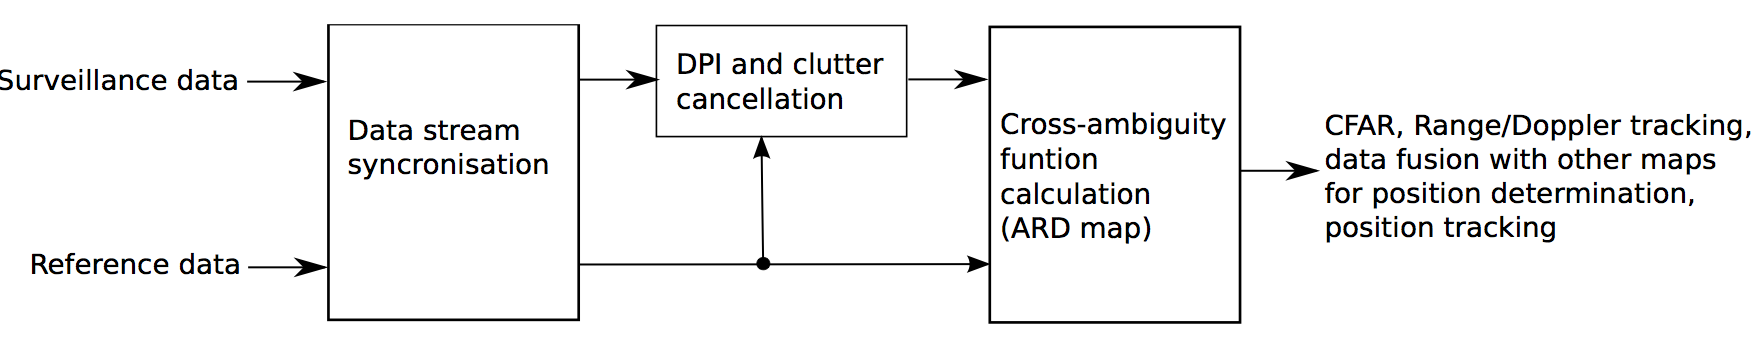
\includegraphics[width=0.8\textwidth, angle=0]{figs/processingChain.png}
\caption{Typical CR processing chain.}
\label{fig:procChain}
\end{center}
\end{figure}

Putative ECM must attempt to interfere with these processing steps. Most repetitive signals, found in both surveillance and reference channels, not exhibiting Doppler, will be removed by the cancellation processing. The output of plots is then shared in the tracking subsystem. Ambiguities inherent in multistatic radar require data from multiple baselines. This is a strength of the tracking process to remove false targets, but a system that is able to overload the tracker with a large number of false targets might have success.

\section{Physical Removal / Destruction of Transmitter / Receivers}

It depends on the level of escalation of a conflict whether the enemy will destroy the transmitters being used by the CR. Clearly, these transmitters are exposed, and can be taken out by obvious means. In this case, the CR cannot operate, unless emergency steps are taken. It is relatively simple for a new transmitter to be deployed (in principle), but it needs to be protected in some way \cite{doh}.

Receive sites can be located by espionage or reconnaissance, and measures taken to remove them. We note elsewhere that the shape of the antenna farm of a receive site is an obvious indication of the frequency of operation to the enemy, and must be protected or spoofed to give the wrong information.

If the transmitters being used by CR system include those from the opposing country, they can be switched off, thereby removing some of the capability of the CR system.

\section{CR Deployment Options}

This topic, as mentioned lies at the root of the difficulty of deploying ECM against CR. Here we look at a few physical layout options, not so much considering the issue of frequency of operation, etc.

\subsection{Fixed Infrastructure CR}

The CR consists of transceivers and receiver sites that are fixed, and carefully designed to meet a required detection requirement. For example, a single receiver site might operate with multiple transmitters. Otherwise, the receivers can be distributed and operate with a single transmitter site. If we include the different frequencies of operation of even a single transmit site, the MIMO nature shows up i.e. N:M.

Such a fixed infrastructure is physically quite vulnerable, especially if the opposition has good prior information. The transmitters being utilised are at risk, especially if the opposition is aware of which frequencies are being utilised. The version that has a single receive and processing centre is especially vulnerable. A spatially distributed network is quite robust, provided the processing centre is safe, and the communications links redundant.

This difficulty that the enemy has in jamming a CR system is demonstrated in figure~\ref{fig:CRdeploy}. The fixed CR system is covering an air corridor from left to right. A single transmitter is used, with rings of receivers to remove ambiguity and improve resolution.

\begin{figure}[htbp]
\begin{center}
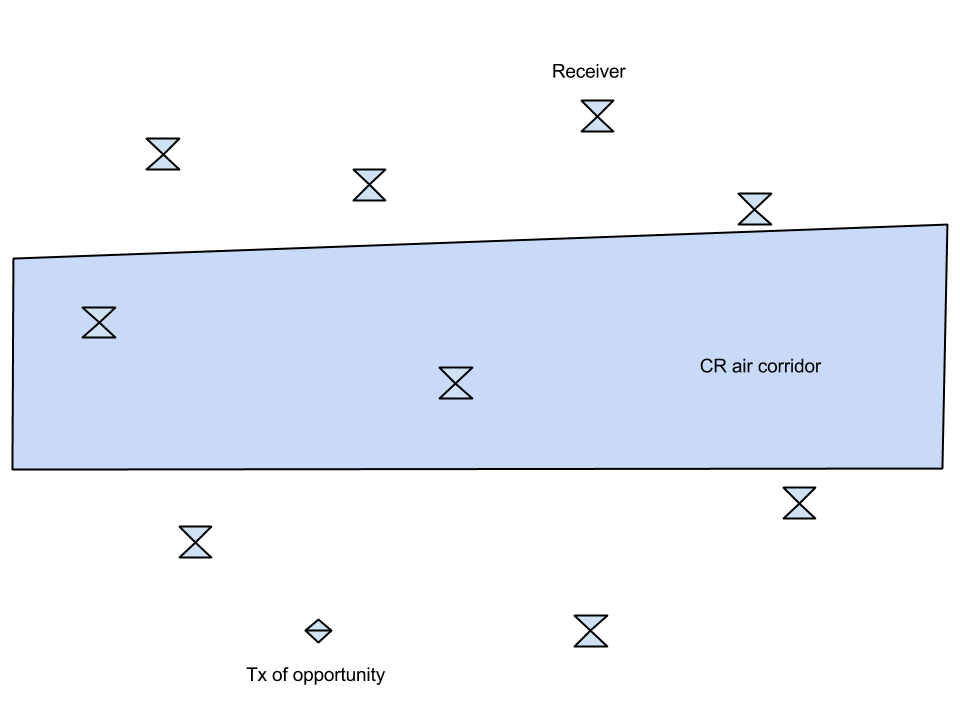
\includegraphics[width=\columnwidth]{figs/CRdeploy}
\caption[Fixed architecture SIMO CR System example][Typical fixed CR system deployment.]{An air corridor from left to right, marked in blue is being surveilled by rings of CR receivers relying on the transmitter designated in the diagram. Typically this figure might represent an area of some 500 by 300 km in extent. Each CR receiver will have its surveillance channel beam (and beamwidth) oriented to cover a portion of the corridor. The reference signal could be distributed via a communications channel based on a receiver protected from jamming. The difficulty of a jammer to position itself to jam all receivers, or, at the majority of them, is clear. A large offset in range is required, further reducing power density, but some of the receivers will always have their beams oriented away from the jammer. Thus the CR system might degrade, but cannot be made totally ineffective.}
\label{fig:CRdeploy}
\end{center}
\end{figure}


\subsection{Mobile Infrastructure CR}

Here the transmitters and / or the receivers of the CR can be mobile. Mobile transmitters are possibly less liable for location and destruction by the enemy, but the moving of the transmitters will make the operation of the CR system quite complex. 

The receivers can be moved without detection by the enemy (other than visual). Again, the reconfiguration of the system will be problematic in operation. In general, it should not be necessary to move receiver sites, unless of course, the CR is part of an advancing force air protection.

A good battlefield communications infrastructure will allow site reconfigurations to be articulated. Possibly reference waveforms for transmitters being utilised can be distributed via a data network, preventing the enemy from jamming CR reference channels. The bandwidth of many CR systems is very low, making this feasible.

We start by looking at the types of jamming (ECM) that are possible. ECCM is the counter to ECM, and is discussed in the next chapter. 


\section{Jamming Techniques}

ECM possibilities against CR is fairly conventional i.e. (1) Noise jamming (Spot or Barrage) and, (2) Other waveforms. It does not seem that any particular waveform will have an advantage over another, provided it is quite large compared to the transmitter of opportunity and the target of interest. CR is very susceptible to jamming signals, as we will demonstrate.

\section{Scenarios}

It is very difficult to cover all possible scenarios for the ECM against the CR equipment, mostly because the variety of CR types and configurations are so large, and their deployment is so varied. CR could, in the future, be a prime sensor for ATC, or Defence, or, it might be a small system being utilised for gap filling. It could also be part of an advancing force, not wanting to carry powerful radar systems, thereby jeopardising the surrounding formations during anti-radiation attack by the opposing force.

\section{Electronic Support Measures (ESM)}

A good jamming system must be supported by ESM to optimise the use of the precious jammer power and its spatial distribution. For CR radar, this is clearly an issue, since the receiver assets of the system are passive, and potentially undetectable. As stated in Willis' book~\cite{willis:07}, the presence of a CR must be determined by:

\begin{quotation}
(a) ..through visual reconnaissance, infiltration, or compromise, or, (b) ..that a covert air defence net must be operating  in the battle area based on unexplained aircraft losses and a priori knowledge that CR has been deployed.
\end{quotation}

Willis also discusses the need for the ESM operator to have excellent knowledge of what transmitters are operating, and whether they are part of the CR system(s) suspected to be operational in an area. The option to locate the transmitter and destroy them also exists, but that clearly announces the intentions of the opposing force.

Given the variety of different CR systems (Bands of operation, combinations of bands, different geometries) the task of the ESM system is very difficult. Only very thorough preparation (as mentioned above) is going to allow the raid planner to be able to decide on the best jamming assets. It is thus crucial that the geometry and type of CR system is kept highly classified.

\section{Discussion from Willis' Book}
\subsection{Noise Jamming}

In Section 6.7 a review is given of ECM and ECCM for ``Passive Bistatic Radar'' (PBR), reflecting only the performance of a single PBR system. This assumption allows for some quantitative assessment, which is very useful, but clearly not the whole story. We take up the key reasoning used by the authors in the next chapter, as well as the chapter on ECCM. Willis goes on to analyse the effectiveness of a CR against noise jamming. The reason is that it is easy to quantify, and not subjected to the variability of all the other techniques mentioned above. This is not to say that these methods are deprecated. The operational planner will need to model the effectiveness of his tactical deployment, and discover a sequence that has a high chance of success. This planning requires access to good simulation capabilities, to carry out a number of putative tactical methods.


\subsection{Effectiveness of Noise Jamming}
 (following [page 172]~\cite{willis:07})
 
To assess the effectiveness of Noise Jamming (NJ) Willis invokes the ``benchmark range'' of the CR. This is:

\begin{description}
\item[First ] 
Find the \emph{benchmark range} of the CR. This is essentially the root of the product of the transmitter-to-target, receiver-to-target range ($R_T , R_R$).
See  equation 6.8 of Chapter 6 of Willis~\cite{willis:07} for a full expression.


\item[Second] Calculate JNR and estimate input noise temperature (using equation 6.54). Being a noise jammer, the effect on the CR is considered to be an addition to the noise temperature.

\item[Third]
Divide Benchmark Range  (first step) by a factory depending on the ratio of the jammer noise to the system noise to see effect on the benchmark range with jamming: equation 6.55.

\item[Fourth]
Assume a specific range difference $\Delta = R_T - R_R$ or just the baseline to set geometry.

\item[Fifth]
Use (3) and (4) and Table 6.5~\cite[ p129]{willis:07} to find Rx to target range and 6.13 to find receiver to target range and coverage area due to the noise jammer.

\end{description}

One can now evaluate various example CR performances. Willis examines an FM transmitter based system (single receiver) working with a 250 kW transmitter, bandwidth 100 kHz. Results are presented in Willis~\cite[pages 175-178]{willis:07}. Two jammer transmitters are considered i.e. 100 W and 1 kW. These results are very unfavourable in terms of predicted reduction in CR performance when the jammer has access to the main beam of the CR. Sidelobe jamming, however, is shown to improve the advantage of the CR system enormously~\cite[Table 6-16)]{willis:07}. This emphasises the advantage of a spatially diverse receiver type of CR, as it will be very difficult for a jammer to come into the main lobe of all receivers.

However, the simulations that we now present show the vulnerability of a CR to jamming, considering a more realistic environment than just noise equivalence, as  shown in the previous analysis. These simulations include real clutter removal, which is not successful in removing the strong clutter signal. This analysis pushes the CR towards only certain types of ECCM i.e. methods that can remove the jamming signal, such as null steering.


\section{Noise Jamming Simulations}

To illustrate the effects of noise jamming on a single CR receiver, a simulation scenario is set up in the Flexible Extensible Radar Simulator (FERS)~\cite{Brooker_FERS:2011,FERS:2013}. The simulation is based on typical deployment geometry as tested in the Western Cape of South Africa around Cape Town. 

\subsection{Simulation overview}
The geometry is illustrated in Figure~\ref{fig:SimGeometryGE}. A receiver is located at the North most region of map labelled Malmesbury Rx. This receiver exploits an FM band transmitter labelled Constantiaberg Tx in the South West corner of the map. A jammer is positioned at a well known high site overlooking the entire region. This is located in the middle of the map. An aircraft flies from the North East which mimics the typical Johannesburg / Cape Town flight path of this region. The aircraft heads towards the Cape Town International Airport, labelled as CPT Airport. The simulation runs for 3 minutes, during which time the aircraft descends from 10000 to 5000~m, travelling at a constant straight line velocity of 200~m/s. 

\begin{figure}[htbp]
\begin{center}
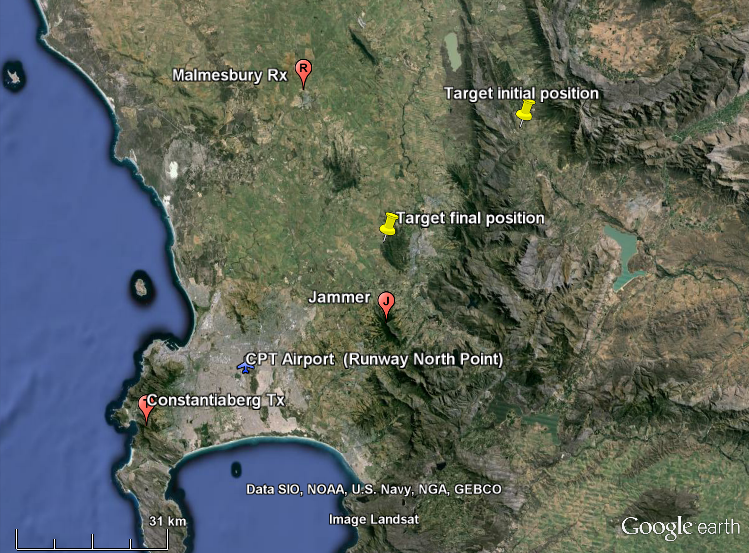
\includegraphics[width=0.8\textwidth]{figs/Simulations/GEGeometryOverview.png}
\caption{An overview of the geometry for jamming simulations. North is upwards.}
\label{fig:SimGeometryGE}
\end{center}
\end{figure}

The Constantiaberg transmitter radiates isotropically for simplicity. The radar receiver has a pair of 60 degree beam-width, 7.2 dBi antennas with a sinc-function based response as shown in Figure~\ref{fig:AntennaBeam} for both vertical and horizontal planes. This is very similar to the Yagi antennas used in the prototype FM band radar at UCT. At the recevier site, the reference antenna points towards the Contastantiaberg transmitter. The surveillance antenna points towards the centre of the target flight path, i.e. between the 2 thumbtacks. The jammer has the same 7.2 dBi antenna as the receiver and points directly towards the receiver. Further details are given in Table~\ref{tab:SimulationParameters}.

\begin{figure}[htbp]
\begin{center}
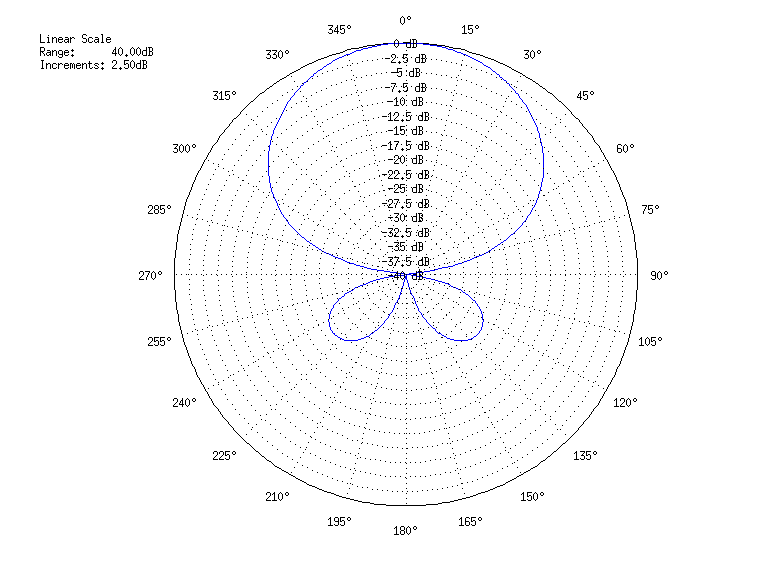
\includegraphics[width=0.9\textwidth]{figs/Simulations/AntennaBeam.png}
\caption[Antenna pattern used in jamming simulations.]{Antenna beam used for the radar receiver and jammer. This pattern applies to both the horizontal and vertical. 0 dB boresight is equivalent to 7.2~dBi gain.}
\label{fig:AntennaBeam}
\end{center}
\end{figure}

\begin{table}[ht!]\label{tab:SimulationParameters}
\caption{Noise jammer simulation parameters.}

	\centering
	
	\vspace{1cm}
	\begin{tabu} to \columnwidth { X r }
  		Item 								& Parameter\\
  		\hline
  		\textbf{Transmitter} 				& \\
  		Antenna beam pattern 				& Isotropic\\
  		Antenna gain 						& 0 dBi\\
  		Antenna altitude 					& 400~m\\
  		Power 								& 16.4~kW (EIRP for 10~kW dipole)\\
  		Carrier frequency					& 89~MHz\\
  		Waveform							& Real recorded FM data 204.8 kSps complex sampled\\[3mm]
  		
  		\textbf{Receiver} 					& \\
  		Antenna beam pattern 				& Sinc\\
  		Antenna gain 						& 7.2 dBi (see Figure~\ref{fig:AntennaBeam})\\
  		Antenna altitude					& 240~m\\
  		LO error							& ~50 ppb (std. dev. of 0.01~Hz @ 204.8 kSps)\\
  		Noise figure						& 4 dB\\
  		Digitisation						& 204.8 kSps complex, 16 bit quantisation\\[3mm]

		\textbf{Target} 					& \\
		Initial altitude					& 10000~m\\
		Final altitude						& 5000~m\\
		Velocity							& Constant 200~m/s\\
		RCS @ 89~MHz						& 46 dBsqm (200~m$^2$, a large airliner)\\[3mm]
		
		\textbf{Jammer} 					& \\
		Antenna beam pattern				& Sinc\\
  		Antenna gain 						& 7.2 dBi (see Figure~\ref{fig:AntennaBeam})\\
  		Transmit power						& 1, 5 and 10~W before antenna gain\\
  		Carrier frequency					& 89 MHz\\
  		Waveform							& 204.8 kSps complex, random noise\\[3mm]
  		
  		\textbf{Radar Signal Processing}	& \\
  		DPI cancellation					& 5 range, 5 Doppler bins\\
  		DPI cancellation CPI				& 102400 samples (0.5~s)\\
  		Range/Doppler processing			& 120 range, 1601 Doppler bins\\
  		Range/Doppler CPI					& 819200 samples (4~s)\\
  		CFAR algorithm						& GOCA-CFAR\\
  		CFAR window							& 4 guards, 8 reference cells (per side of CUT)\\
  		CFAR dimension						& Doppler (robust against bandwidth fluctuations)\\
  		CFAR threshold					    & P$_{fa}$ = 10$^{-5}$ (exponential noise model)\\
				  
	\end{tabu}
	
	\vspace{1cm}
	
\end{table}

\subsection{Illuminating Signal of Opportunity}
The illuminating signal of opportunity used in the simulation is real FM data recorded at the actual site on which the simulation is based. This site has a favourable interference environment and is relatively free of multipath. The data is stored as a complex baseband stream of IQ data sampled at 204.8 kSps. It is fed into the simulator in this form. The simulator software mixes the baseband data up to a carrier frequency of interest. This way the simulation will produce realistic bandwidth functions in the FM band signal as well as a realistic FM signal ambiguity function. The spectrum and ambiguity function of the FM signal are shown in Figures~\ref{fig:FMFrequencyResponse} and~\ref{fig:JammerAAF} respectively.

\begin{figure}[htbp]
\begin{center}
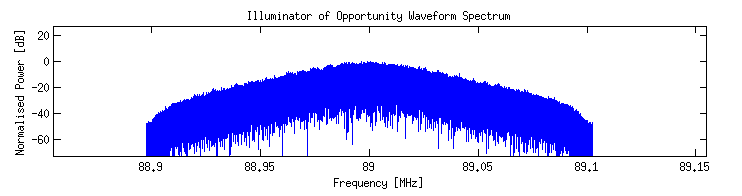
\includegraphics[width=0.9\textwidth]{figs/Simulations/FMSpectrum.png}
\caption{The spectrum of the illuminator of opportunity (FM) signal shown at its RF frequency.}
\label{fig:FMFrequencyResponse}
\end{center}
\end{figure}

Observing the shape of the spectrum in Figure~\ref{fig:FMFrequencyResponse}, it is clear that the average modulation bandwidth of the signal falls below 204.8 kHz. Typically the FM standard allows for up to 150~kHz with the average being closer to 80~kHz in practice for a typical music radio programme. Furthermore, if one inspects the equation for processing gain as shown in Equation~\ref{equ:ProcessingGain}, a maximum modulation bandwidth of 204.8 kHz in the 204.8 KSps complex data block would allow for an integration gain of around 60~dB assuming a 4 second integration time, as is consistent with such an FM band radar.

\begin{align}\label{equ:ProcessingGain}
G_{int} & = t_{int} \cdot \beta\\
	    & = 10 \log{\bigg(4~s \cdot 204.8~kHz\bigg)}\\
	    & = 59.13~dB
\end{align}

Where $G_{int}$ is integration gain, $t_{int}$ is the integration time and $\beta$ is the bandwidth of the signal.

Observing the auto-ambiguity function in Figure~\ref{fig:FMAAF} it is apparent that the integration peak at 0~range, 0~Doppler is approximately 50~dB above the surrounding background. This processing gain will reduce further for coherent processing intervals (CPIs) that have an even lower average modulation bandwidth as would be the case, for example, during a broadcast of speech over the duration of the CPI.

Also related to the modulation bandwidth is the range resolution. As can be observed the 0~range, 0~Doppler peak extends over several range bins. This relation is governed by Equation~\ref{equ:BistaticRangeRes}. In the case of the simulation which uses a 204.8~kSps (complex) signal and a carrier frequency of 89~MHz, the bin resolutions will be 1463.83~m and 0.25~Hz for bistatic range and bistatic Doppler resolutions respectively. 0.25~Hz is equivalent to 0.84~m/s bistatic range rate at 89~MHz.

\begin{equation}\label{equ:BistaticRangeRes}
\Delta R = \frac{c}{\beta \cos{  (\theta / 2 )}}
\end{equation}

Where $\Delta R$ is the attainable bistatic range resolution in metres (which applies to the same dimension as bistatic range), $c$ is the speed of light in metres per second, $\beta$ is the instantaneous modulation bandwidth of the signal that is being exploited in Hertz and $\theta$ is the bistatic angle, that is, the angle formed by the transmitter-target and target-receiver line segments in radians. The minimum distance to which two separate targets can be told apart will therefore be approximately twice that of the bistatic range resolution.

\begin{figure}[htbp]
\begin{center}
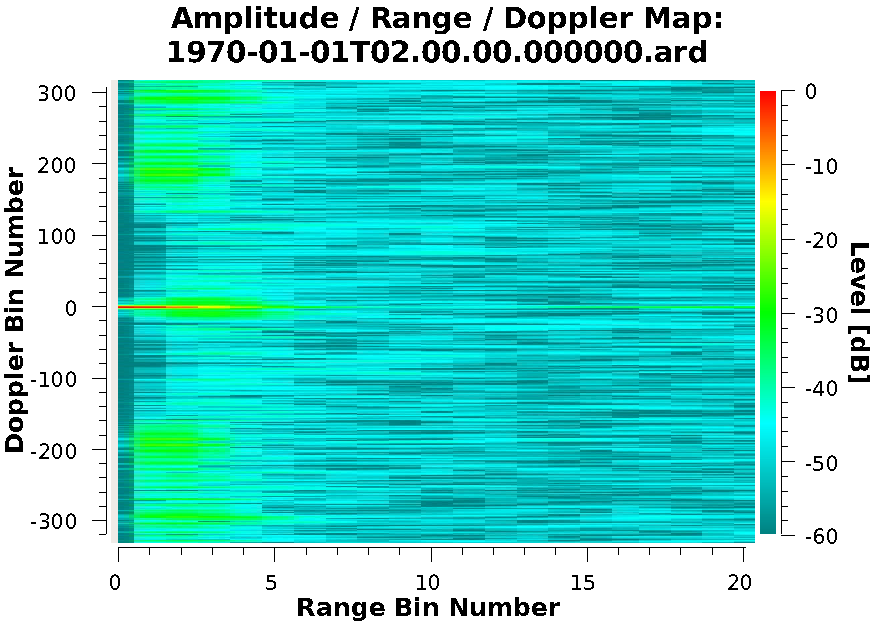
\includegraphics[width=0.9\textwidth]{figs/Simulations/FMAAF.pdf}
\caption{Normalised auto-ambiguity function of illuminator of opportunity (FM) jammer signal.}
\label{fig:FMAAF}
\end{center}
\end{figure}

\subsection{Jamming Signal}
The jamming signal is generated as a complex 204.8 kSps random sequence, which, as such occupies the full bandwidth of the target FM channel. The spectrum of the signal as mixed to a 89 MHz carrier is shown in Figure~\ref{fig:JammerFrequencyResponse}. The flat frequency response is characteristic of the noise-like time domain signal, occupying 204.8 kHz of bandwidth. In practice the response of the RF frontend would attenuate the edge of the frequency pedestal.

\begin{figure}[htbp]
\begin{center}
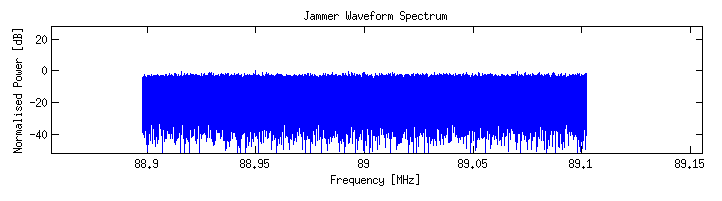
\includegraphics[width=0.9\textwidth]{figs/Simulations/JammerSpectrum.png}
\caption{The spectrum of the jamming signal shown at its RF frequency.}
\label{fig:JammerFrequencyResponse}
\end{center}
\end{figure}

The auto-ambiguity function of the jammer signal, which is the cross-ambiguity function of the jamming signal with itself, is shown in Figure~\ref{fig:JammerAAF}. This is calculated for an integration period of 819200 samples which is in line with the processing interval of a long range FM band CR. As can be seen, the function produces a ``thumbtack'' reponse which can be attributed to the critically sampled noise signal that the jammer emits. Only a small extent of range and Doppler bins are displayed to show the detail of the peak but the background noise will extend for all practical ranges. Furthermore, because the signal content is a full 204.8~KHz, the integration peak to noise ratio of the ambiguity function is the maximum $\sim$60~dB which agrees with the formula for integration gain (shown in Equation~\ref{equ:ProcessingGain}). As with the FM signal the bin resolutions will be 1463.83~m and 0.25~Hz for bistatic range and bistatic Doppler resolutions respectively because the sample rate is the same. 0.25~Hz is again equivalent to 0.84~m/s bistatic range rate at 89~MHz. The difference here is that because the jamming signal is critically sampled, the integration peak will tend not to span multiple range bins. This would therefore be a highly desirable waveform to exploit for radar operation should the power be sufficient and the transmitter location be known.

\begin{figure}[htbp]
\begin{center}
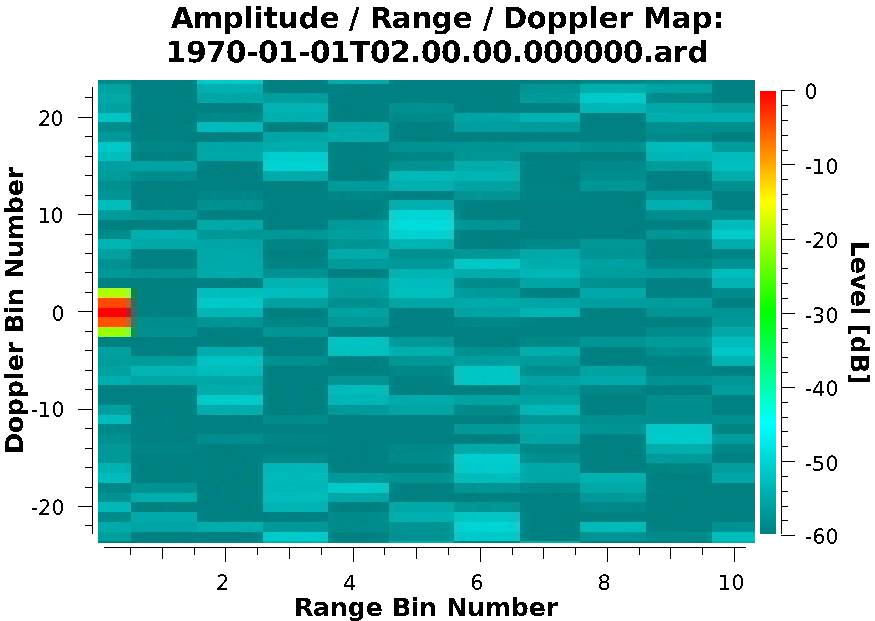
\includegraphics[width=0.9\textwidth]{figs/Simulations/JammerAAF.pdf}
\caption{Normalised auto-ambiguity function of the jammer signal.}
\label{fig:JammerAAF}
\end{center}
\end{figure}

A passive radar receiver that receives such a jamming signal on both it's surveillance and reference channel would therefore suffer integrated interference across its range/Doppler plane as shown by Figure~\ref{fig:JammerAAF}. The peak level would be scaled according to the received signal strength at the receiver input.

\subsection{Simulation Runs}\label{sec:ECMSims}
The following runs are performed with the FERS simulator to gauge the effect of the jammer on the radar. For all the simulations presented here, the signal level of the plot has been normalised to the level of the target at the beginning of the first clean simulation run as shown in Figure~\ref{fig:NoJammingARDFirst} of the simulation without jamming. This way the noise and interference floor level can be compared directly to the signal level of the target return.

\subsubsection{No Jamming}
To establish a performance baseline a simulation with the target flying its specified trajectory with no interfering signal present is also performed.

The target displays a signal to noise ratio in the range of 25~to~30~dB for the duration of manoeuvre. This is consistent with actual measurements taken at the site exploiting the same transmitter and observing large commercial airliners flying along a similar trajectory. Figure~\ref{fig:NoJammingARDFirst} shows the range/Doppler map at the beginning of the target manoeuvre, Figure~\ref{fig:NoJammingARDLast} shows the range/Doppler map at the end of the target manoeuvre and Figure~\ref{fig:NoJammingCFAR} shows the CFAR filter detection history for all frames of the target manoeuvre.

\begin{figure}[htbp]
\begin{center}
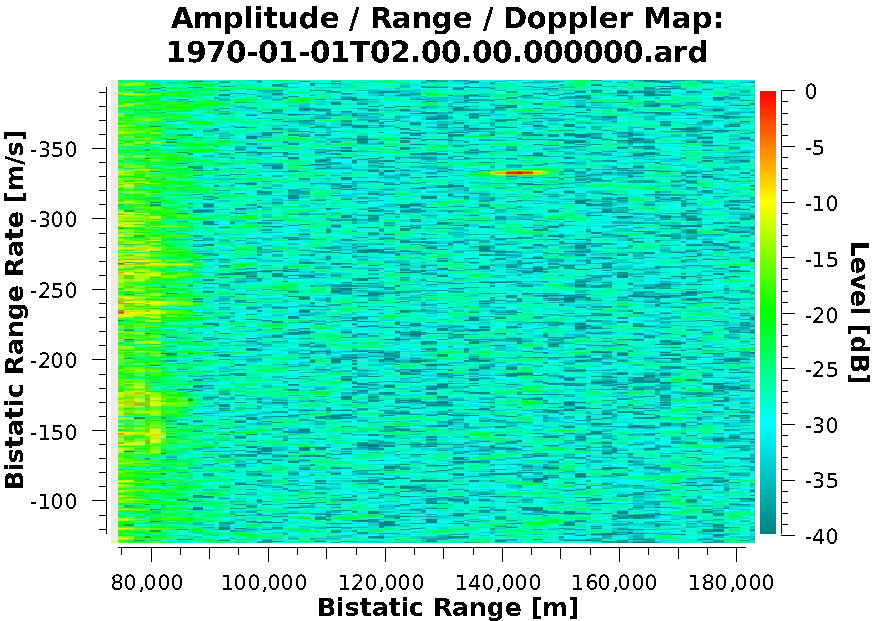
\includegraphics[width=0.7\textwidth]{figs/Simulations/NoJammingARDFirst.pdf}
\caption{ARD at the beginning of the flight trajectory when no jamming is present.}
\label{fig:NoJammingARDFirst}
\end{center}
\end{figure}

\begin{figure}[htbp]
\begin{center}
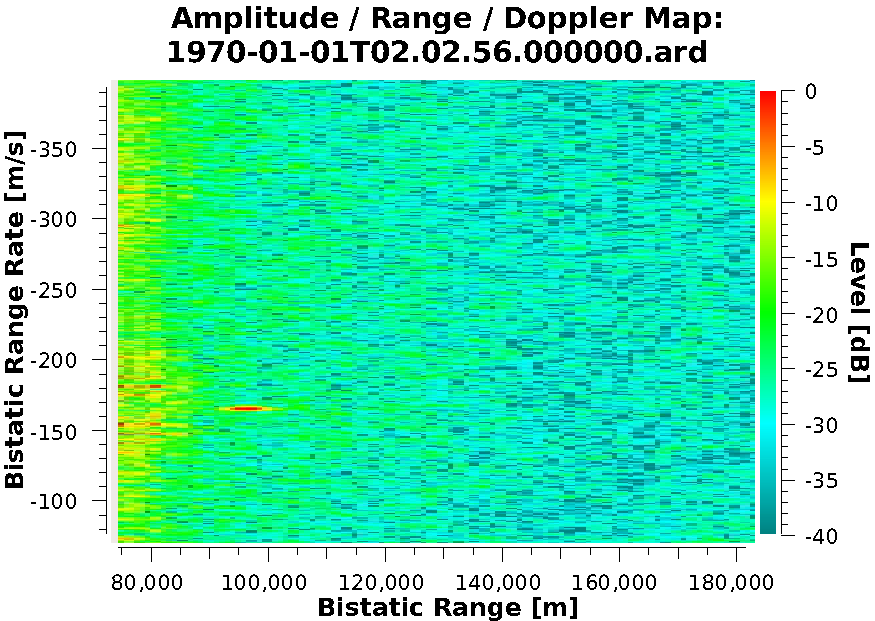
\includegraphics[width=0.7\textwidth]{figs/Simulations/NoJammingARDLast.pdf}
\caption{ARD at the end of the flight trajectory when no jamming is present.}
\label{fig:NoJammingARDLast}
\end{center}
\end{figure}

\begin{figure}[htbp]
\begin{center}
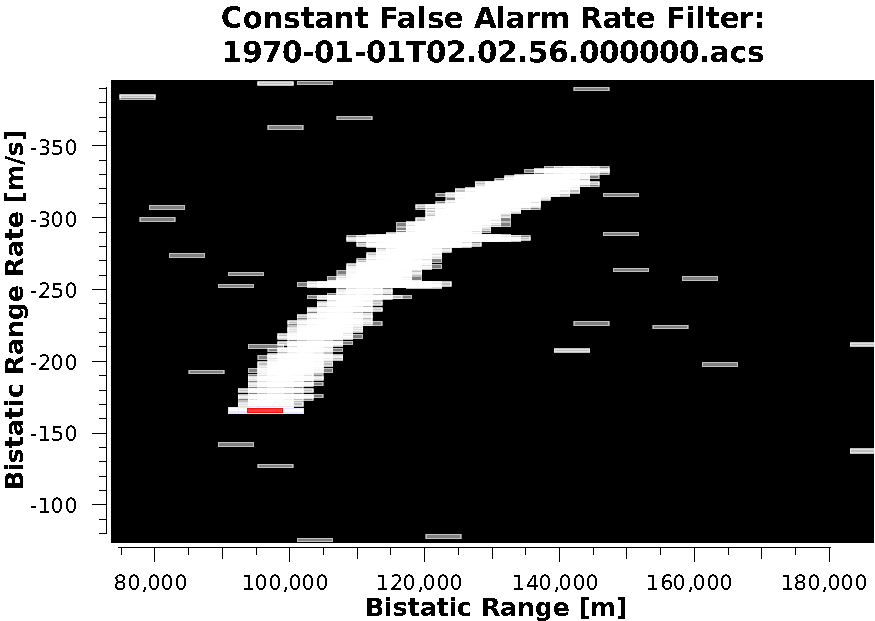
\includegraphics[width=0.7\textwidth]{figs/Simulations/NoJammingCFAR.pdf}
\caption{CFAR history for the duration of the flight trajectory when no jamming is present.}
\label{fig:NoJammingARDCFAR}
\end{center}
\end{figure}

\clearpage

\subsubsection{1W Jamming}
The jammer is now activated with 1 W of power feeding into the 7.2 dBi antenna which is directed at the radar receiver site. There is a noticeable rise in the noise floor and accordingly a drop in SINR, approximately 10~dB. The CFAR filter is still able to detect the target through the manoeuvre. Figure~\ref{fig:1WJammingARDFirst} shows the range/Doppler map at the beginning of the target manoeuvre, Figure~\ref{fig:1WJammingARDLast} shows the range/Doppler map at the end of the target manoeuvre and Figure~\ref{fig:1WJammingCFAR} shows the CFAR filter detection history for all frames of the target manoeuvre.

\begin{figure}[htbp]
\begin{center}
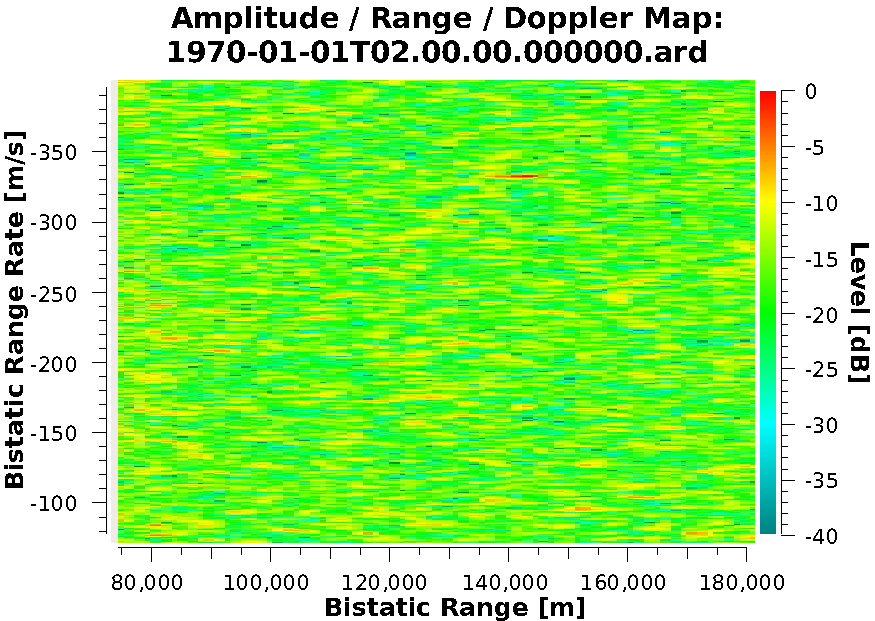
\includegraphics[width=0.7\textwidth]{figs/Simulations/1WJammingARDFirst.pdf}
\caption{ARD at the beginning of the flight trajectory when 1~W jamming is present.}
\label{fig:1WJammingARDFirst}
\end{center}
\end{figure}

\begin{figure}[htbp]
\begin{center}
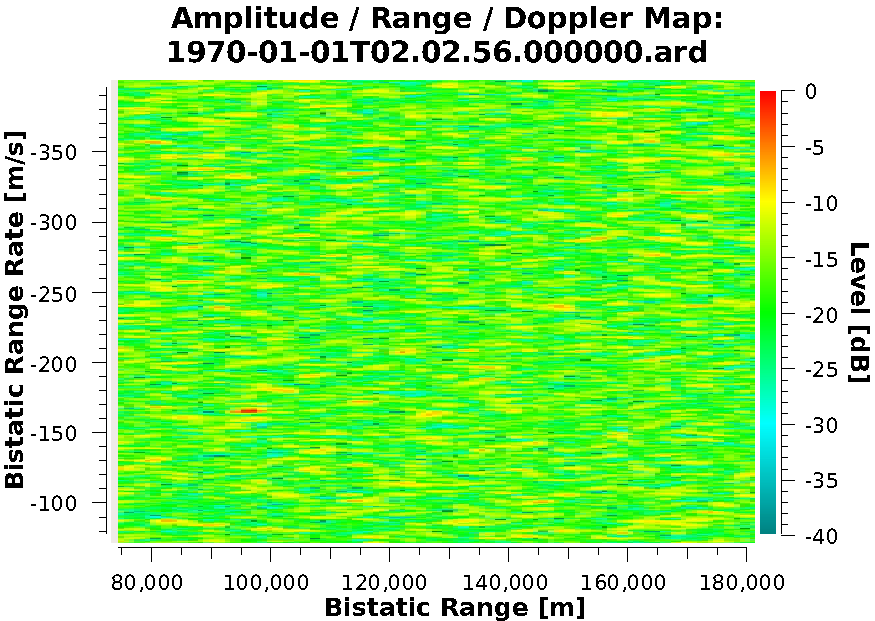
\includegraphics[width=0.7\textwidth]{figs/Simulations/1WJammingARDLast.pdf}
\caption{ARD at the end of the flight trajectory when 1~W jamming is present.}
\label{fig:1WJammingARDLast}
\end{center}
\end{figure}

\begin{figure}[htbp]
\begin{center}
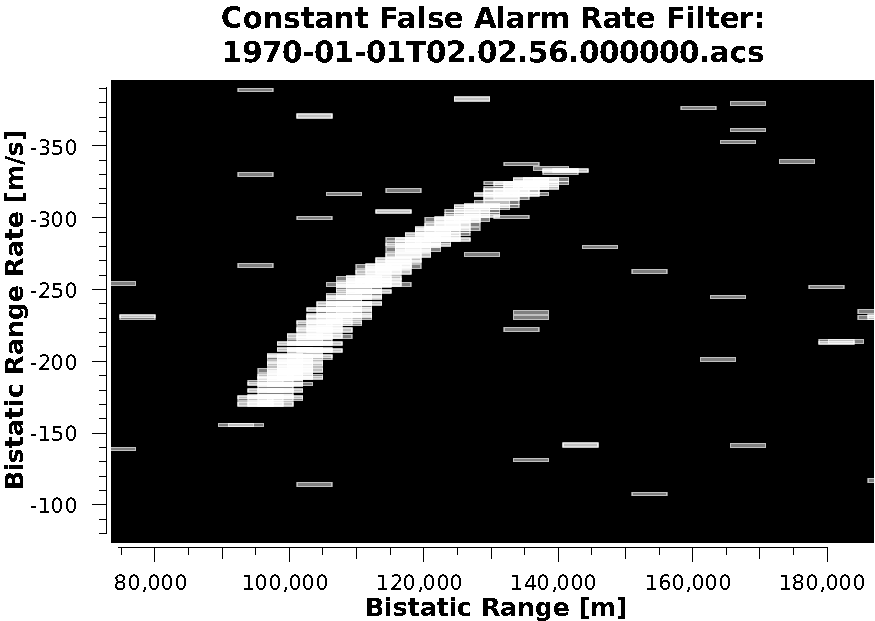
\includegraphics[width=0.7\textwidth]{figs/Simulations/1WJammingCFAR.pdf}
\caption{CFAR history for the duration of the flight trajectory when 1~W jamming is present.}
\label{fig:1WJammingARDCFAR}
\end{center}
\end{figure}

\clearpage

\subsubsection{5W Jamming}
The noise jammer power is increased to 5 W. The target is no longer discernible even when viewing successive ARD maps in sequence. The interference floor is raised by another 6~dB approximately which is equivalent to the doubling of power impinging on the 2 antennas of the radar. The CFAR detector produces a vague suggest as to the flight path but this would likely be insufficient to drive a tracking filter. Figure~\ref{fig:5WJammingARDFirst} shows the range/Doppler map at the beginning of the target manoeuvre, Figure~\ref{fig:5WJammingARDLast} shows the range/Doppler map at the end of the target manoeuvre and Figure~\ref{fig:5WJammingCFAR} shows the CFAR filter detection history for all frames of the target manoeuvre.

\begin{figure}[htbp]
\begin{center}
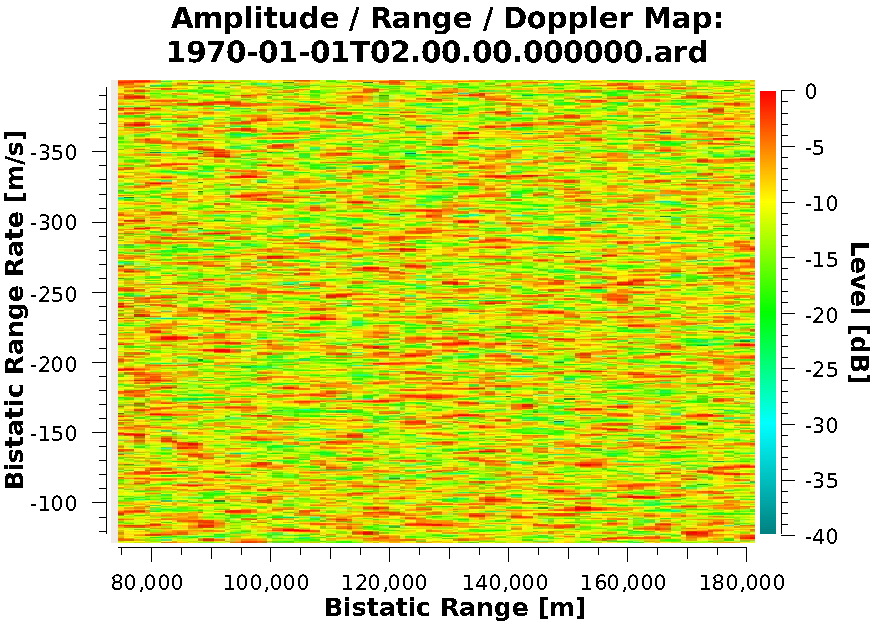
\includegraphics[width=0.7\textwidth]{figs/Simulations/5WJammingARDFirst.pdf}
\caption{ARD at the beginning of the flight trajectory when 5~W jamming is present.}
\label{fig:5WJammingARDFirst}
\end{center}
\end{figure}

\begin{figure}[htbp]
\begin{center}
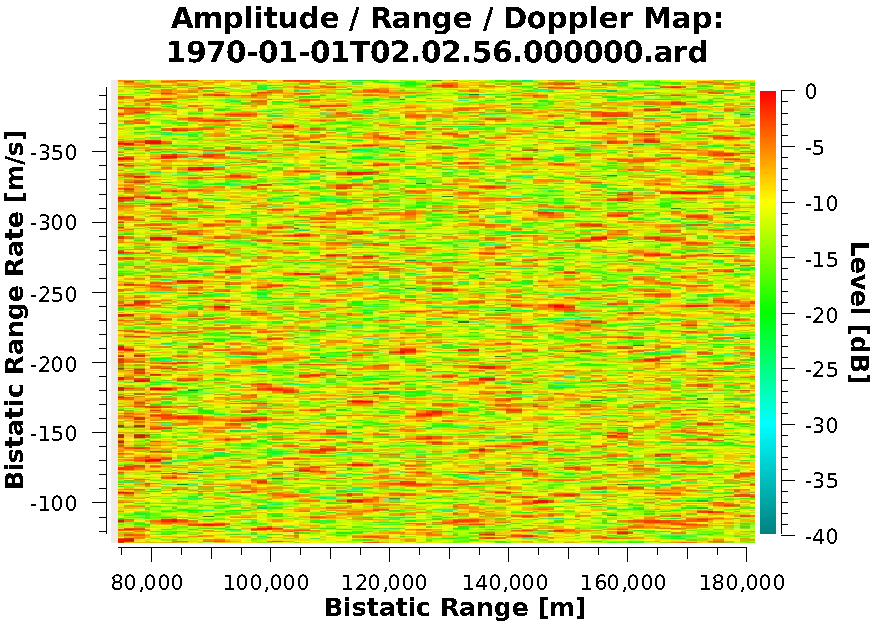
\includegraphics[width=0.7\textwidth]{figs/Simulations/5WJammingARDLast.pdf}
\caption{ARD at the end of the flight trajectory when 5~W jamming is present.}
\label{fig:5WJammingARDLast}
\end{center}
\end{figure}

\begin{figure}[htbp]
\begin{center}
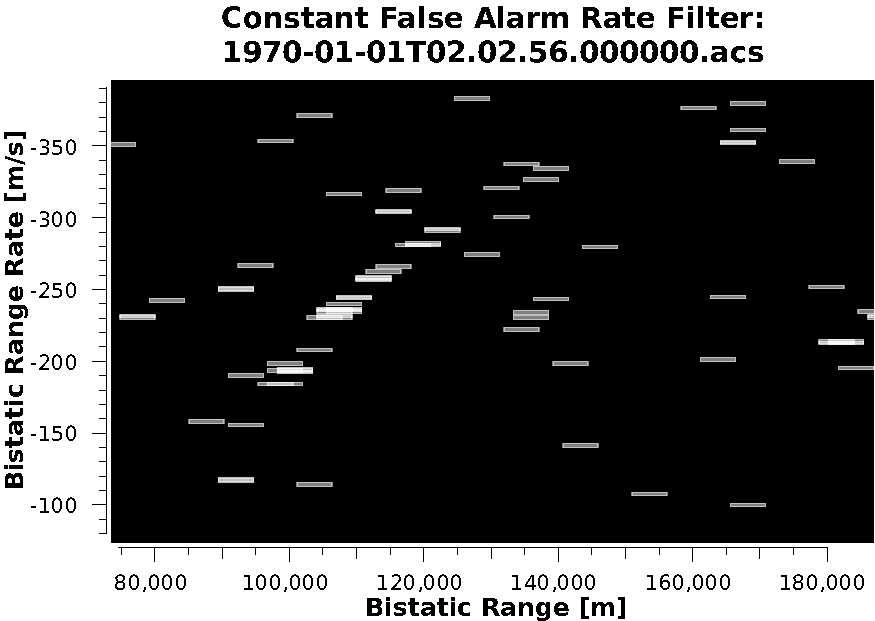
\includegraphics[width=0.7\textwidth]{figs/Simulations/5WJammingCFAR.pdf}
\caption{CFAR history for the duration of the flight trajectory when 5~W jamming is present.}
\label{fig:5WJammingARDCFAR}
\end{center}
\end{figure}

\clearpage

\subsubsection{10W Jamming}\label{sec:Jam10W}
The noise jammer power is then increased to 10 W. The target is no longer discernible in a single stationary ARD map. The interference floor is raised by another 10~dB approximately. The CFAR detector begins to loose a significant number of detections during the target manoeuvre. Figure~\ref{fig:10WJammingARDFirst} shows the range/Doppler map at the beginning of the target manoeuvre, Figure~\ref{fig:10WJammingARDLast} shows the range/Doppler map at the end of the target manoeuvre and Figure~\ref{fig:10WJammingCFAR} shows the CFAR filter detection history for all frames of the target manoeuvre.

\begin{figure}[htbp]
\begin{center}
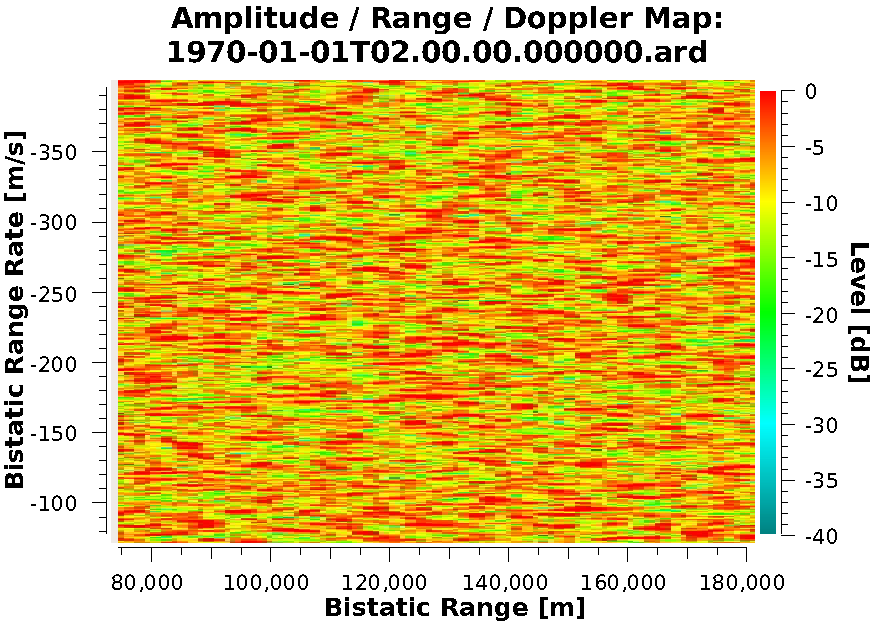
\includegraphics[width=0.7\textwidth]{figs/Simulations/10WJammingARDFirst.pdf}
\caption{ARD at the beginning of the flight trajectory when 10~W jamming is present.}
\label{fig:10WJammingARDFirst}
\end{center}
\end{figure}

\begin{figure}[htbp]
\begin{center}
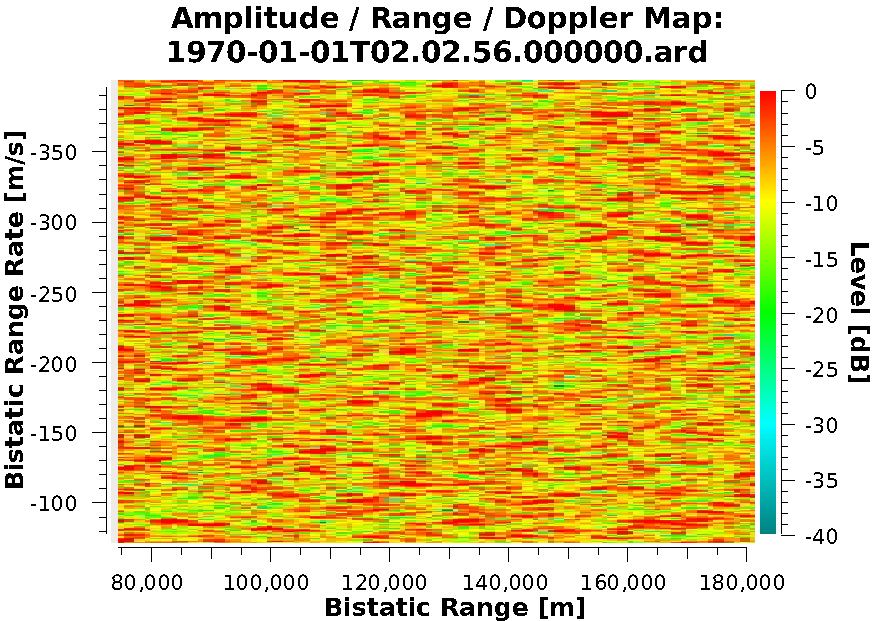
\includegraphics[width=0.7\textwidth]{figs/Simulations/10WJammingARDLast.pdf}
\caption{ARD at the end of the flight trajectory when 10~W jamming is present.}
\label{fig:10WJammingARDLast}
\end{center}
\end{figure}

\begin{figure}[htbp]
\begin{center}
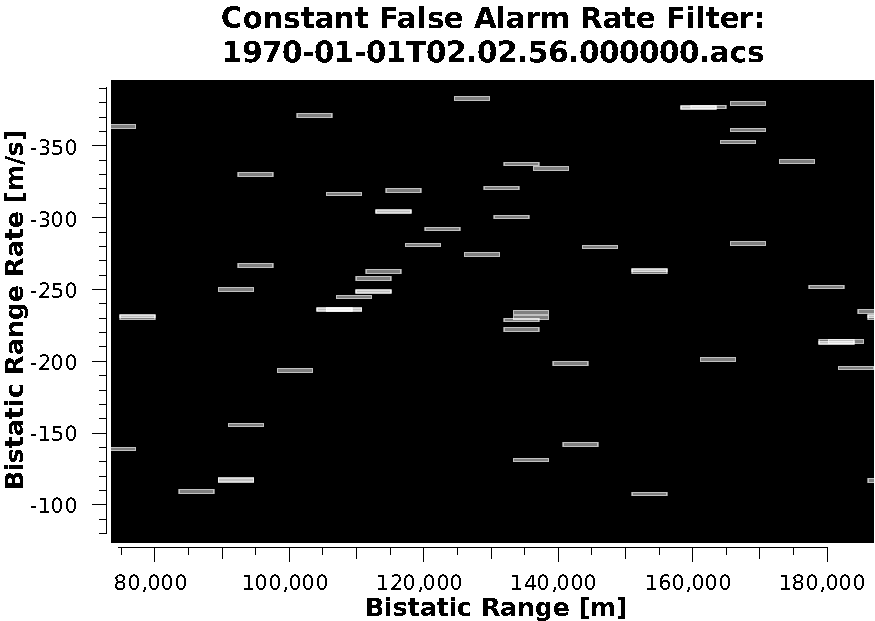
\includegraphics[width=0.7\textwidth]{figs/Simulations/10WJammingCFAR.pdf}
\caption{CFAR history for the duration of the flight trajectory when 10~W jamming is present.}
\label{fig:10WJammingCFAR}
\end{center}
\end{figure}

\clearpage

\subsubsection{Target Self-protection}\label{sec:SelfProtection}

This section discussed the implications of the target radiating its own jamming signal. This is simulated with an omni-directional beam pattern. Only 1 W of power is radiated given that airborne ECM platforms are likely to have power limitations.

Figures~\ref{fig:1WSelfProtectionARDFirst} and~\ref{fig:1WSelfProtectionARDLast} show the ARD output for the 1 W transmitter though an omni directional antenna on the target aircraft. In effect the emitted signal is orders of magnitude larger than the target echo even at only 1~W and so masks the radar return effectively. Figure~\ref{fig:1WSelfProtectionCFAR} shows the CFAR trail for the entire trajectory. The target trajectory is not identifiable in the output map.

\begin{figure}[htbp]
\begin{center}
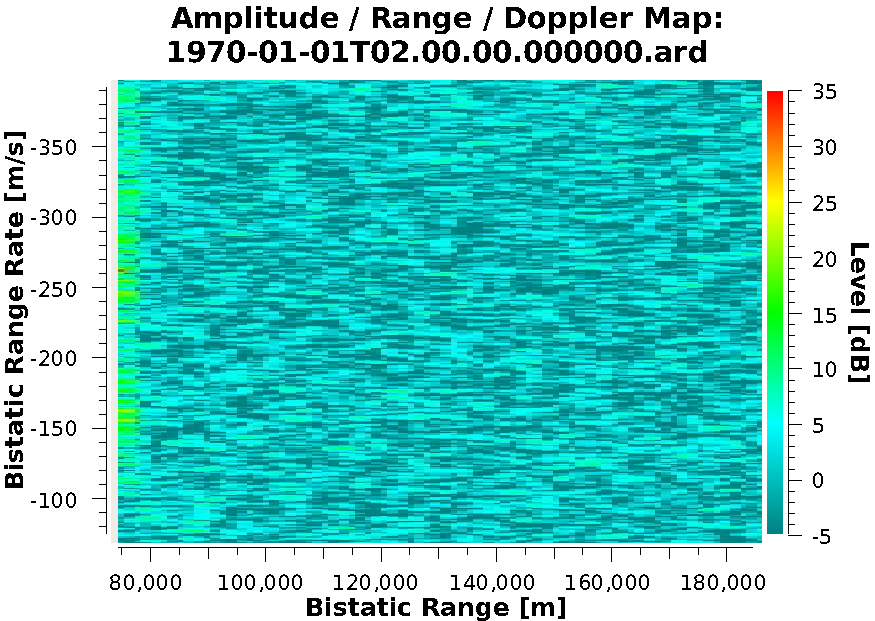
\includegraphics[width=0.7\textwidth]{figs/Simulations/1WSelfProtectionARDFirst.pdf}
\caption{ARD at the beginning of the flight trajectory when 1~W self-protection jamming from the target is present.}
\label{fig:1WSelfProtectionARDFirst}
\end{center}
\end{figure}

\begin{figure}[htbp]
\begin{center}
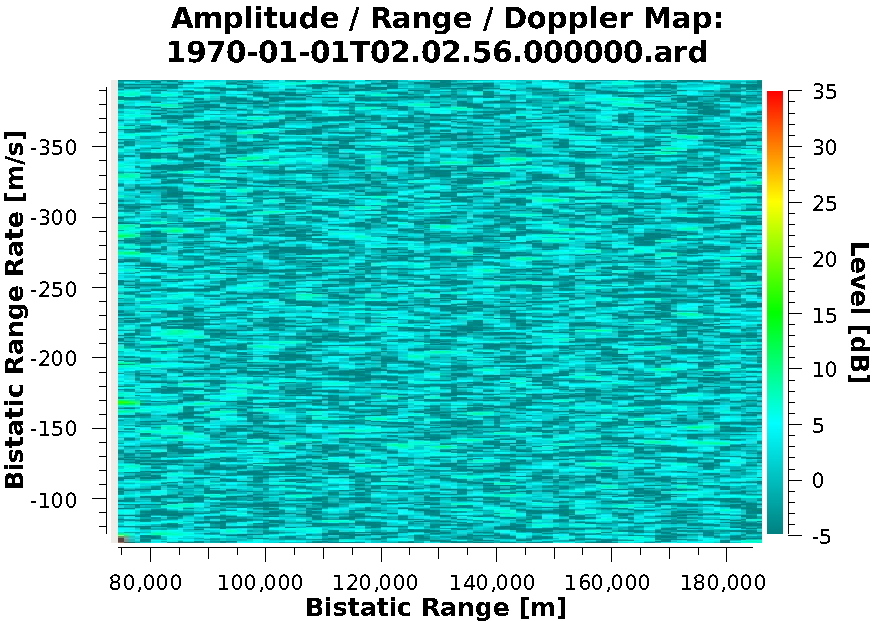
\includegraphics[width=0.7\textwidth]{figs/Simulations/1WSelfProtectionARDLast.pdf}
\caption[1~W self-protection jamming from the target is present]{ARD at the end of the flight trajectory when 1~W self-protection jamming from the target is present.}
\label{fig:1WSelfProtectionARDLast}
\end{center}
\end{figure}

\begin{figure}[htbp]
\begin{center}
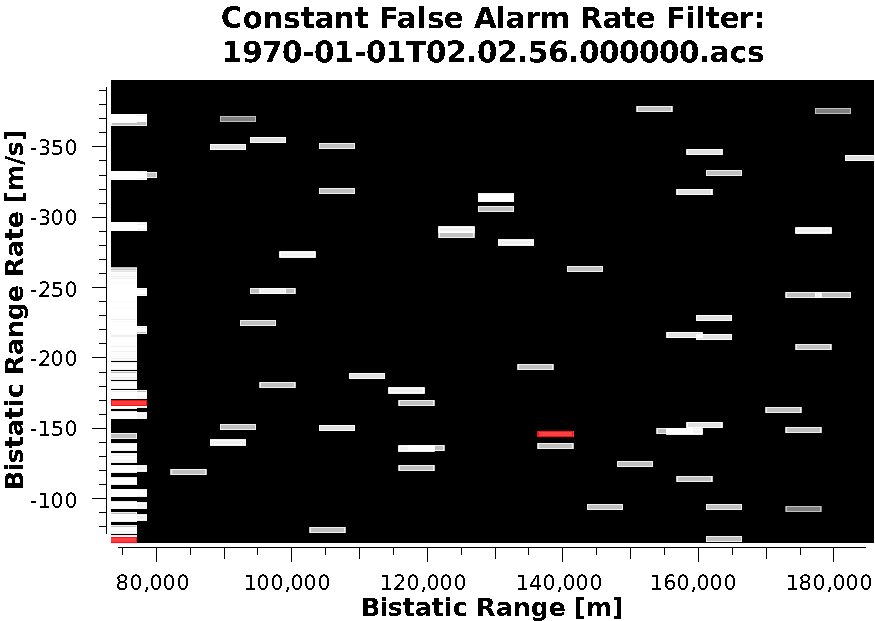
\includegraphics[width=0.7\textwidth]{figs/Simulations/1WSelfProtectionCFAR.pdf}
\caption[CFAR 1~W self-protection jamming from the target. ]{CFAR history for the duration of the flight trajectory when 1~W self-protection jamming from the target is present.}
\label{fig:1WSelfProtectionCFAR}
\end{center}
\end{figure}

To further investigate the effect of self protection jamming, the ARD map shown at the beginning of the trajectory as in Figure~\ref{fig:1WSelfProtectionARDFirst} is normalised to the level of the target return. The target return level is again derived as the jamming free interference simulation run as shown in Figure~\ref{fig:NoJammingARDFirst}. The normalised version of Figure~\ref{fig:1WSelfProtectionARDFirst} is shown in Figure~\ref{fig:1WSelfProtectionARDFirst_targetNormalised}. As can be observed the noise-plus-interference floor now sits some 20~dB above the level of the target, meaning detection is highly unlikely.

\begin{figure}[htbp]
\begin{center}
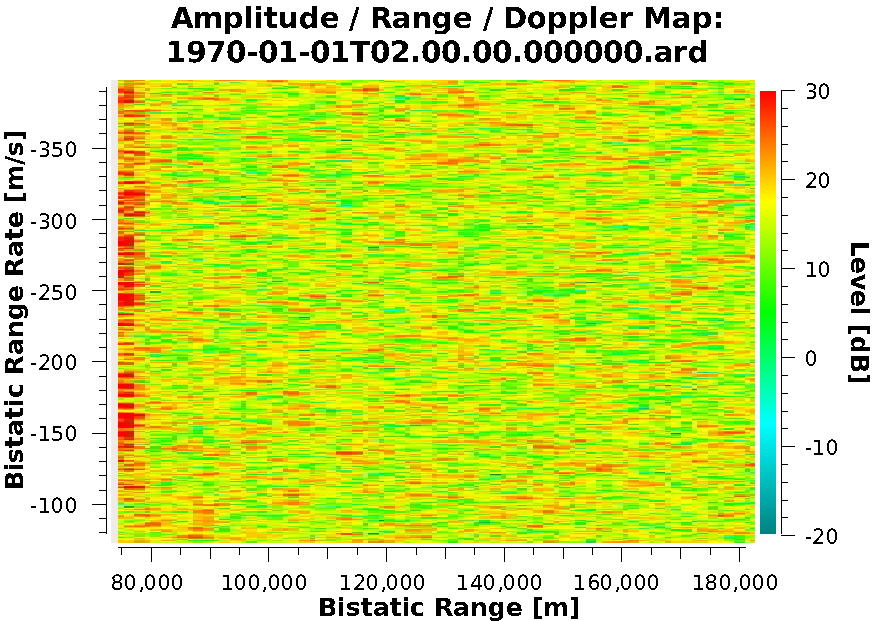
\includegraphics[width=0.7\textwidth]{figs/Simulations/1WSelfProtectionARDFirstTargetNormalised.pdf}
\caption[ARD map normalised to target return.]{ARD at the beginning of the flight trajectory when 1~W self-protection jamming from the target is present. The map is normalised to the level of the target return.}
\label{fig:1WSelfProtectionARDFirst_targetNormalised}
\end{center}
\end{figure}

\clearpage


\section{Spot versus Barrage Jamming}

A CR system, working with a large number of channels in the FM Band, for example, will force the jammer to cover the whole of the FM Band, if the jammer does not know which specific transmitters are being utilised. This is an advantage to the CR system. If the jammer knows exactly which transmitters are being utilised, with sophistication can schedule its power only where required, i.e. more energy per jammed channel. We point out that modern signal processing hardware allows a CR system to use a large number of channels.

\section{Conclusions}

This chapter has explored the effectiveness of ECM deployed again a CR. After some general comments about the difficulty faced by the ECM operator, we demonstrate with a number of simulations the effectiveness of ECM when the CR system's positions are known. The effectiveness of a self-protection jammer is also shown.

%================================
\chapter{Electronic Counter-countermeasures (ECCM) for CR}
%================================

 Here we examine techniques which could protect passive radars against
 
 \begin{itemize}
\item  jamming / interfering transmitters ,
\item recognition of wrong targets,
\item sector blanking,
\item Chaff,
\item Decoys,
\item Deception waveforms, what is the effectiveness of the interfering transmitter that emits the original broadcast signals with time delays and / or Doppler shifts (repeater techniques (DRFM jamming)
\end{itemize}

A big consideration for all ECM techniques is the multistatic geometry (multiple angle illumination of targets by the CR), and the unknown transmitter of opportunity.

Many of the ideas mentioned here are untested: there are just too few CR systems available, and the user has not made credible attempts to firstly, test the effectiveness of a CR system, and then, to test ECM effectiveness and then, appropriate ECCM. For example, we are not aware of a single, long terms deployment of a CR system to actually measure parameters such as $p_d$, $p_{fa}$, cumulative statistics, coverage, etc.

An overriding consideration (philosophy) of ECCM is that it should make the ECM against the CR too expensive to deploy, or, at least very uncertain of its success. Unless the military commander deploying ECM is convinced of its effectiveness, he will be reluctant to deploy assets that are not going to be protected with certainty.

\section{Derivation of the Reference Signal}

A CR system has to have a reference signal that is referenced geographically with respect to the transmitter being utilised for detection. This is often derived via a separate reference channel at the receiver site. Care must be exercised with multipath contamination. A reference signal contaminated with large multipath can lead to ghost targets as well as causing degrading effects on the ARD surface during clutter cancellation~\cite{UCT_SepRefResults:2013}.

The reference signal is cross correlated with the surveillance channel of the receiver. The surveillance channel has an antenna that is pointing towards the region of interest in terms of potential targets. This beam \todo{A little ambiguity here - does "This" refer to the ref. or surv. beam??} can also be the most vulnerable in terms of jamming signals.

Another method is that the reference signal is distributed by network, from a single receiver that is carefully chosen to provide a reference signal [single]. This reference could be provided in a collusion with the broadcaster, and in a sense makes the system \emph{symbiotic}, as discussed in the introduction on Taxonomy.

Some benefits of using a separate site for exclusive capture of the reference signal are discussed. The results presented are from real data acquired during deployment of the prototype FM band commensal radar developed at UCT. In certain scenarios a particular deployment site may have desirable characteristics for the surveillance channel. These characteristic might include good aspect of the airspace volume to be surveyed, low DPI level, access to antenna mast infrastructure, power, telecommunications etc. This site however may not be well suited for capture of the reference signal. Reasons might include, line of sight to the transmitter being exploited, or high levels of multipath. Both of these are likely in mountainous regions.

The Tygerberg site in the Western Cape of South Africa serves as an example of such a site. It has an excellent aspect of incoming and outgoing air traffic to Cape Town International Airport, however the site suffers from a large amount of multiple path at a particular range. The cause of this is shown in Figure~\ref{fig:TygerbergMulipathStructures}. Plotting a 60~km iso-bistatic-range contour for the Tygerberg transmitter and receiver site shows that every significant topographical structure in the region begins near to this range.

\begin{figure}[ht]
\centering
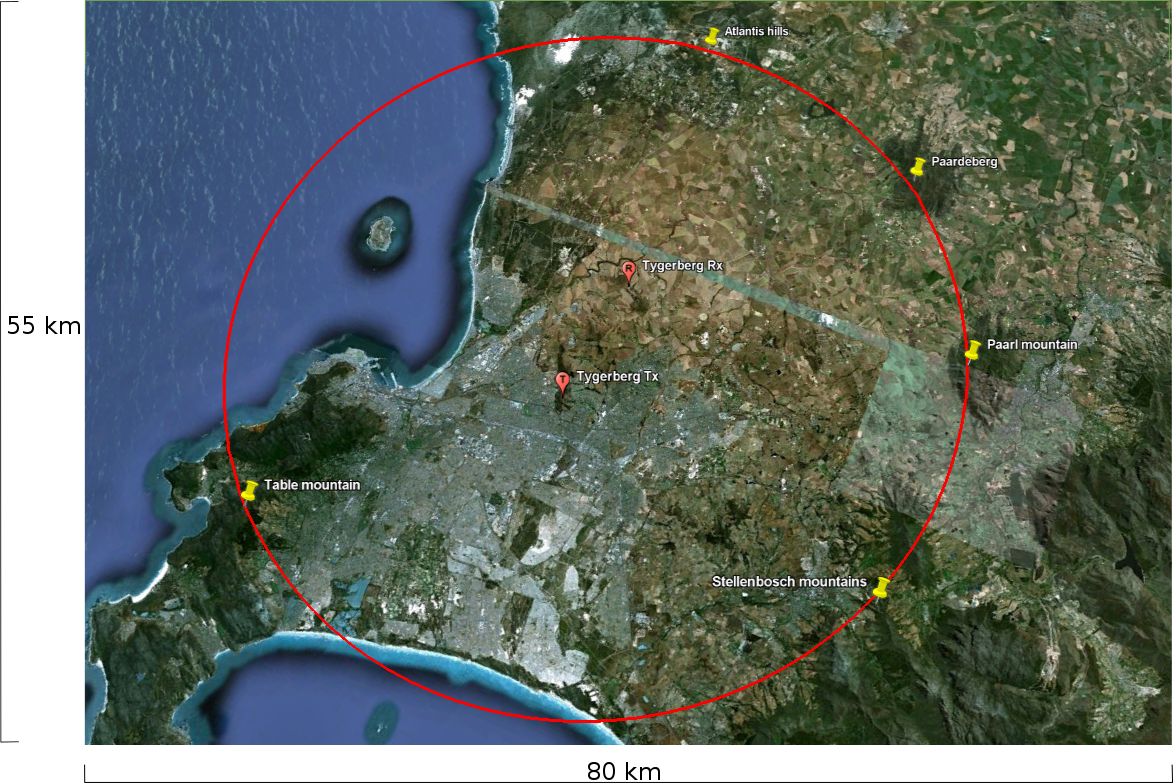
\includegraphics[width=1\columnwidth]{figs/60kmMultipath.png}
\caption[The Tygerberg receive site with multipath]{The Tygerberg receive site has good aspect of the predominant flight path to the North-East but it suffers from severe multipath effects at 60 km bistatic range due to many large terrain structures lying at this range as shown by the red ellipse and thumbtacks.}
\label{fig:TygerbergMulipathStructures}
\end{figure}

Inspecting the auto-ambiguity function of the reference signal captured the Tygerberg receiver site in Figure~\ref{fig:AAFCompare}, it is clear that a secondary peak exists at 60~km due to this multipath effect. Comparing Tygerberg to another receiver site at Malmesbury, which is known to have a cleaner interference environment, (to the North, not shown on the map) it is clear that Malmesbury provides a better reference signal.

\begin{figure}[ht]
\centering
\subfloat[]{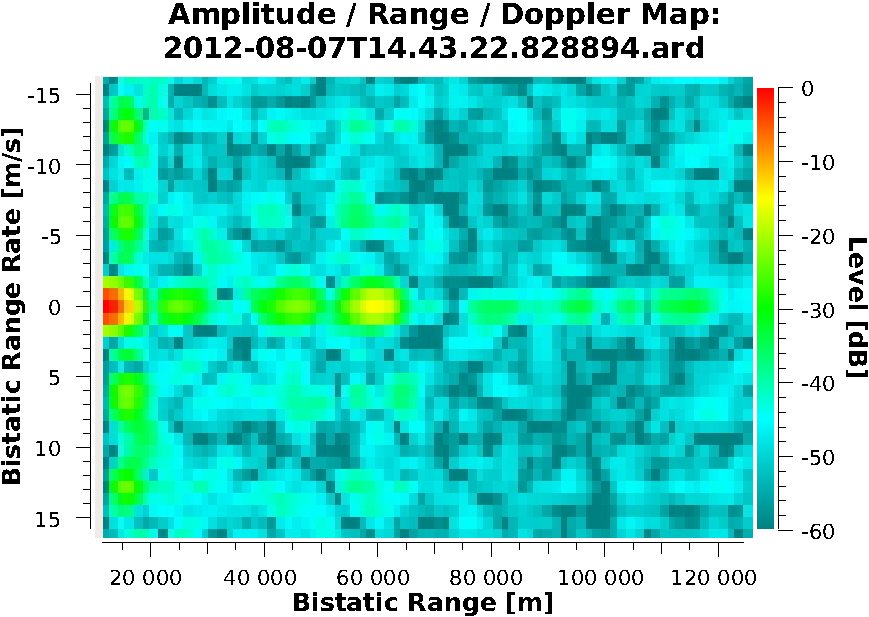
\includegraphics[width=0.5\columnwidth]{figs/TygerbergReferenceAAF1.pdf}}
\hfill
\subfloat[]{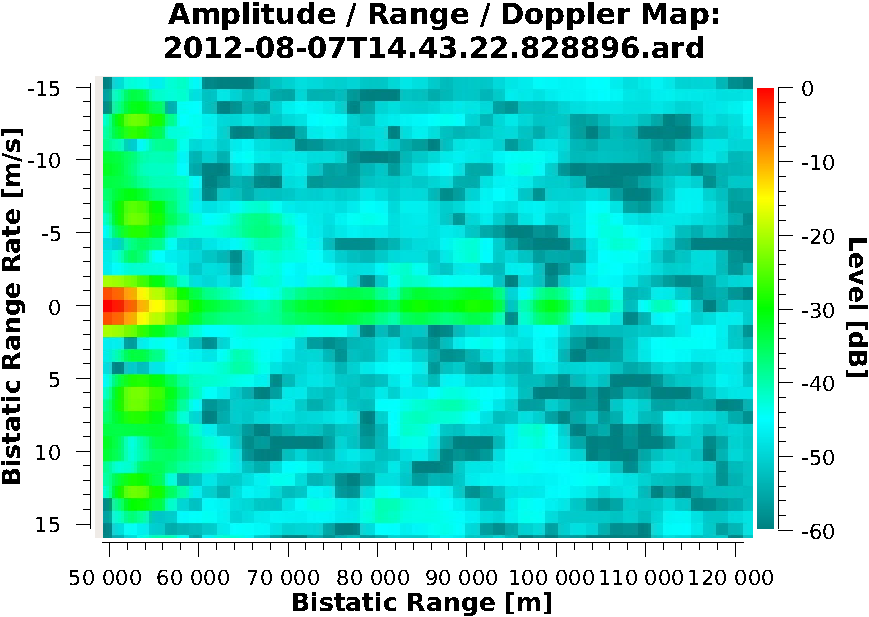
\includegraphics[width=0.5\columnwidth]{figs/MalmesburyReferenceAAF1.pdf}}
\caption[Comparison of ARD maps of the AAF of the reference signals for 2 different receiver sites]{Comparison of ARD maps of the AAF of the reference signals for two different receiver sites. (a) shows the Tygerberg site and (b) the Malmesbury site which has the cleaner reference signal.}
\label{fig:AAFCompare}
\end{figure}

Inspecting radar detection output of the radar in Figure~\ref{fig:MultipathGhostingRemoval} where the surveillance signal is recorded at Tygerberg and the reference is taken either from Tygerberg or Malmesbury, it is clear that the high level of multipath in the Tygerberg reference channel causes target ghosting with an additional detection trail shown 60~km to the right of the true trail. This ghosting is due to the secondary correlation peak in the reference channel data. Such an output as in Figure~\ref{fig:MultipathGhostingRemoval} would cause confusion for a tracking algorithm and invariably cause incorrect radar output. However, when using the cleaner reference signal from Malmesbury, the target ghosting problem is completely removed.

\begin{figure}[ht]
\centering
\subfloat[]{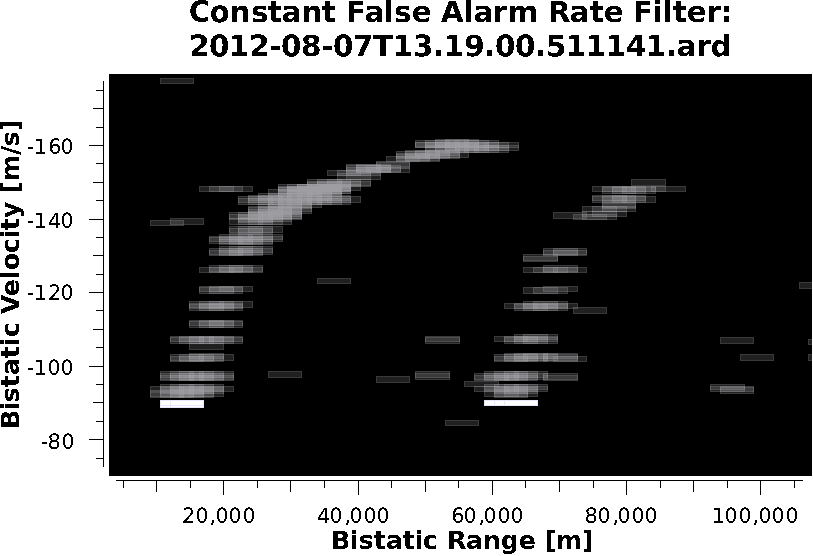
\includegraphics[width=0.7\columnwidth]{figs/CFAR_multipath.pdf}}
\hfill
\subfloat[]{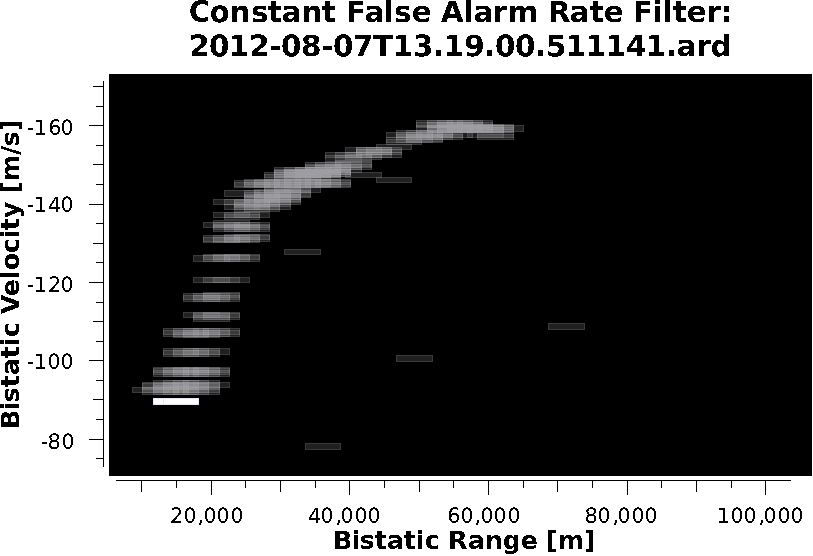
\includegraphics[width=0.7\columnwidth]{figs/CFAR_multipathRemoved.pdf}}
\caption[CFAR with ghost targets]{CFAR detections with the co-located configuration show target ghosting created by the large multipath returns at 60 km bistatic range at the Tygerberg receiver site.}
\label{fig:MultipathGhostingRemoval}
\end{figure}

The next concern about multipath in the reference channel is degradation of the ARD surface due to application of the DPI and clutter suppression filter. This adaptive filter assumes that the reference is free of multipath and builds a vector of weights of the reference signal which is subtracted from the surveillance signal to remove DPI and clutter components. Multipath in the reference signal corrupts the model and introduces unwanted and extraneous components of the reference signal into the interference estimation which is then incorrectly subtracted from the surveillance channel. Figures~\ref{fig:DetectionRangeColocated} and~\ref{fig:DetectionRangeSepRef} show a comparison of maximum detection range where SINR is the critical factor. As with the ghost example, the surveillance channel is taken from the Tygerberg site and the reference channel is used either in co-located configuration, i.e. also recorded at Tygerberg or otherwise recorded separately at the Malmesbury site which provides a cleaner version of the signal. As can be seen the separated reference again provides better performance with a longer detection range indicating that the multipath in the reference signal degrades the SINR of the ARD surface.

\begin{figure}[ht]
\centering
\subfloat[]{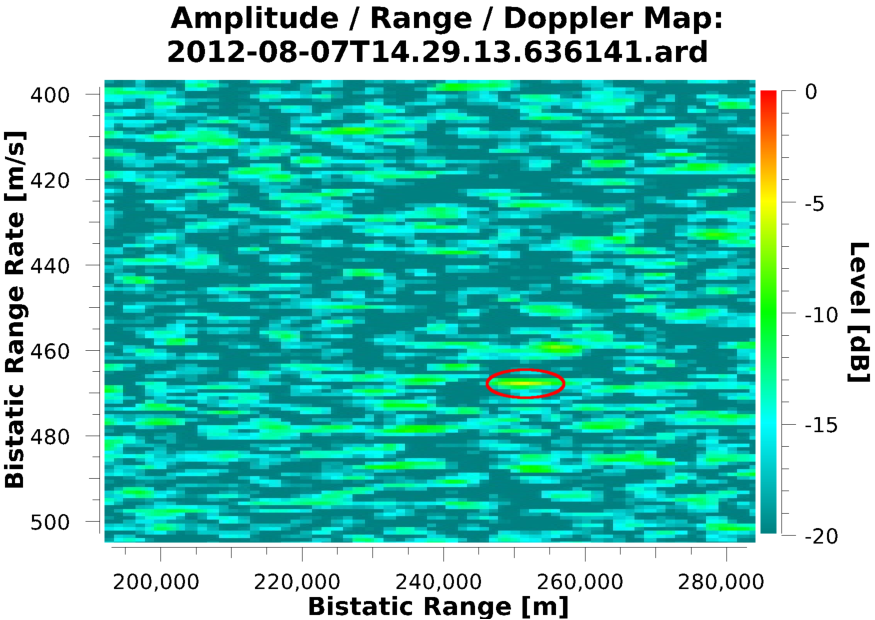
\includegraphics[width=0.5\columnwidth]{figs/CoLocatedMaxDetectionARD.pdf}}
\hfill
\subfloat[]{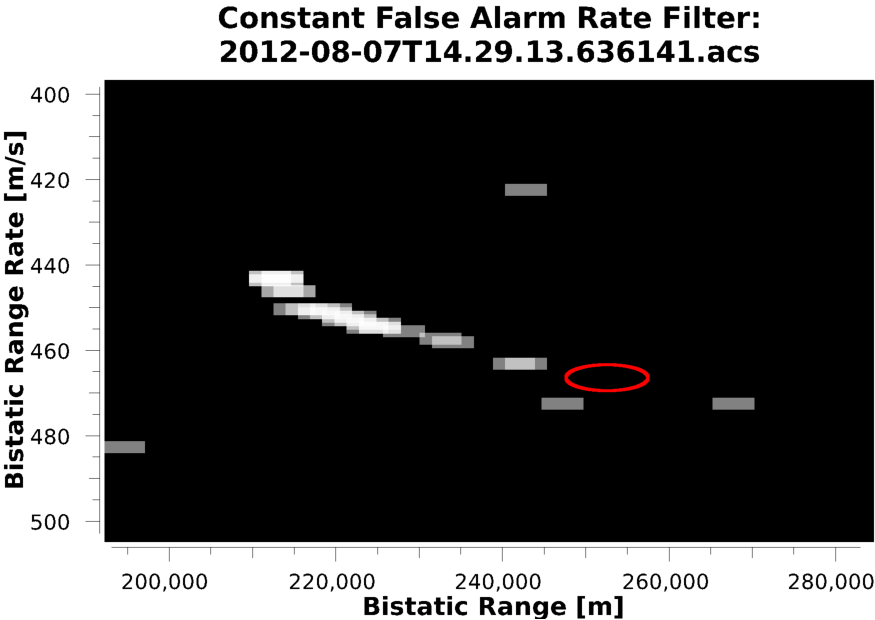
\includegraphics[width=0.5\columnwidth]{figs/CoLocatedMaxDetectionCFAR.pdf}}
\hfill
\caption[Detections of a target at its furthest detectable range using the co-located configuration.]{Detections of a target at its furthest detectable range using the co-located configuration. Figure (a) shows the ARD and gives and indication of the poor SINR. Figure (b) shows the corresponding CFAR. All detections shown are from previous CPI and detection in the current CPI should be within the red ellipse. The SINR is however too poor for the CFAR detector to detect.}
\label{fig:DetectionRangeColocated}
\end{figure}

\begin{figure}[ht]
\centering
\subfloat[]{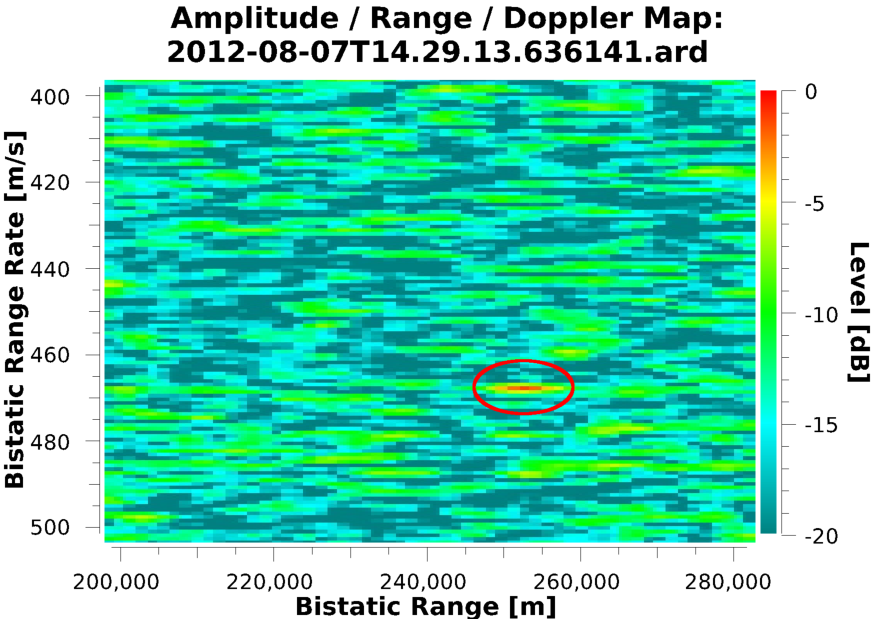
\includegraphics[width=0.5\columnwidth]{figs/SepRefMaxDetectionARD.pdf}}
\hfill
\subfloat[]{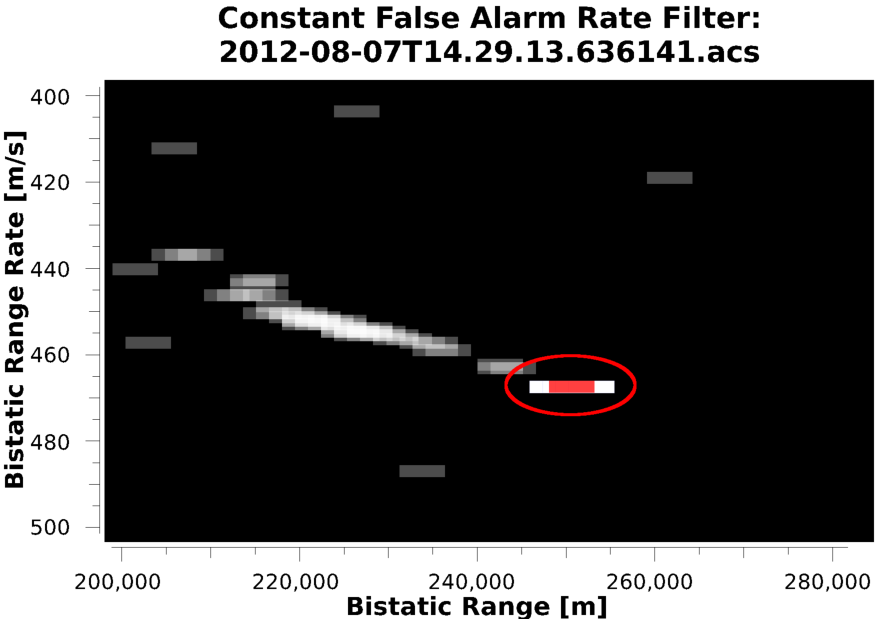
\includegraphics[width=0.5\columnwidth]{figs/SepRefMaxDetectionCFAR.pdf}}
\hfill
\caption[Detection ranges with the separated reference.]{Detection ranges with the separated reference. Using the same surveillance channel at in Figure~\ref{fig:DetectionRangeColocated} with a cleaner reference signal yields similar detection performance. The maximum range is actually increased which can be attributed to improved SINR as shown in Figure (a). Figure (b) now shows a detection in current CPI as indicated within the red ellipse.}
\label{fig:DetectionRangeSepRef}
\end{figure}

\clearpage

As demonstrated, the purity of the reference signal is important, so it should be carefully scrutinised for the presence of jamming. In principle, the jamming signal in the time reference will be cross correlated with the signal in the surveillance channel, and reduce the SNR heavily.

It would thus seem that DPI and clutter suppression by means of an adaptive filter, as is necessary when exploiting FM signals is not a robust method for jamming reduction.

It may be theorised that having a perfectly clean reference channel may protect the radar against noise jamming as the jamming signal in the surveillance channel will not correlate with the reference channel. It can, however, be shown that the general rise in the interference-plus-noise floor by jamming noise in the surveillance channel is enough to mask target detection. To illustrate this, simulations from Section~\ref{sec:ECMSims} are extended. Firstly, a clean copy of the 1 0W jamming signal as digitised by the surveillance antenna of the scenario demonstrated in Section~\ref{sec:Jam10W} is cross calculated in a cross-ambiguity function with a clean version of the reference FM signal as received by the reference channel. This is shown in Figure~\ref{fig:FMJamCAF}. This map has again been normalised to the level of the target in Figure~\ref{fig:NoJammingARDFirst} to be directly comparable to a typical target level. As can be observed, much of the interference-plus-noise floor exists at 0 dB relative to the target which will make target detection no better than having the jammer impinging on both antennas as in the case of Section~\ref{sec:Jam10W}. In fact, the DPI cancellation is likely to remove some component of the jamming signal from the surveillance signal if there is a component in the reference signal and, as such, the case described in Section~\ref{sec:Jam10W} may likely describe a scenario with slightly greater SINR.

\begin{figure}[htbp]
\begin{center}
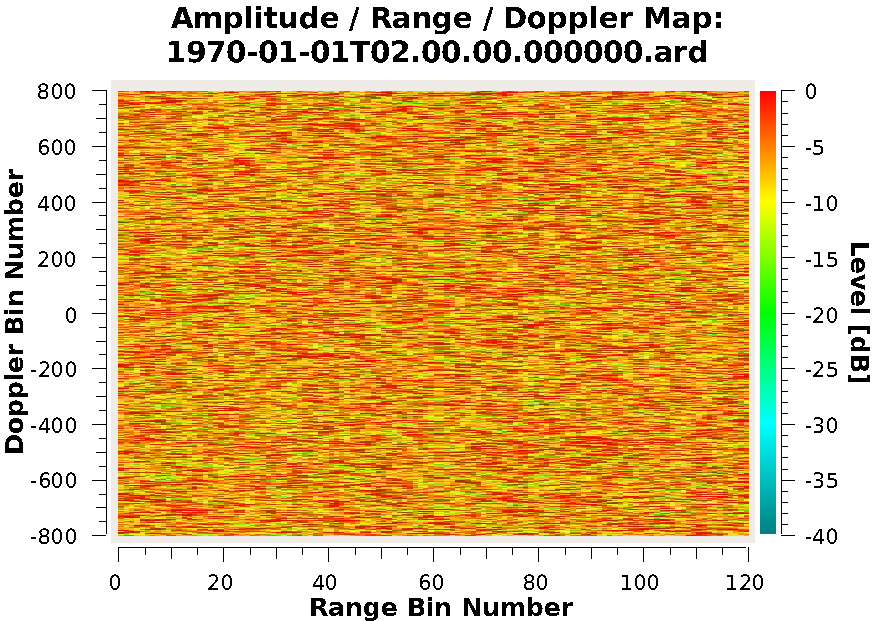
\includegraphics[width=0.7\textwidth]{figs/Simulations/FMJamCAF.pdf}
\caption[Cross ambiguity of jammer and signal]{Cross ambiguity function of the jamming signal and the illuminator of opportunity (FM)signal normalised to target level in Figure~\ref{fig:NoJammingARDFirst} where no jamming is present.}
\label{fig:FMJamCAF}
\end{center}
\end{figure}

To further illustrate this point the simulation from Section~\ref{sec:Jam10W} is rerun with a perfectly clean reference signal where no jamming would be present. Again, Figure~\ref{fig:10WJammingPerfectRefARDFirst} shows the range/Doppler map at the beginning of the target manoeuvre, Figure~\ref{fig:10WJammingPerfectRefARDLast} shows the range/Doppler map at the end of the target manoeuvre and Figure~\ref{fig:10WJammingPerfectRefCFAR} shows the CFAR filter detection history for all frames of the target manoeuvre.

\begin{figure}[htbp]
\begin{center}
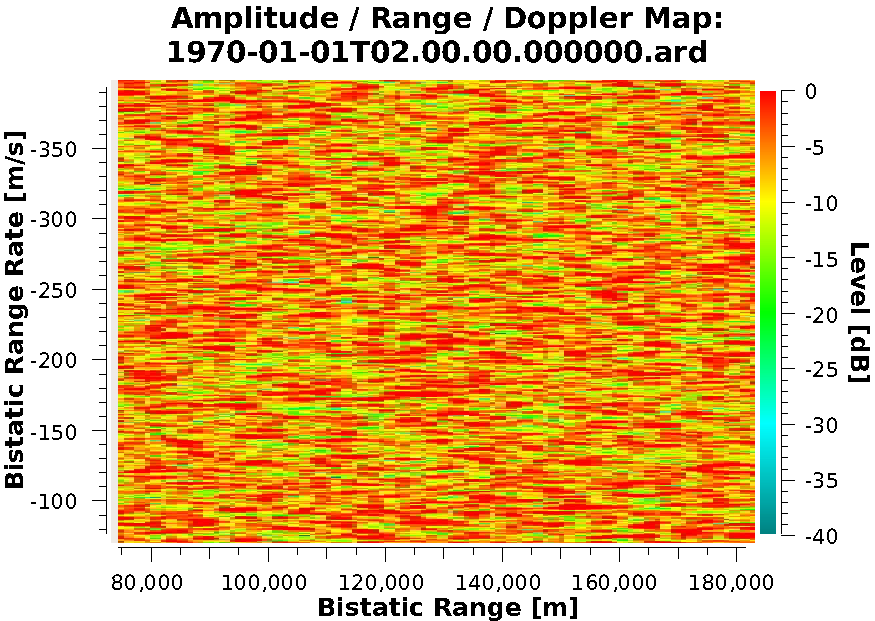
\includegraphics[width=0.7\textwidth]{figs/Simulations/10WJammingPerfectRefARDFirst.pdf}
\caption[ARD at the beginning of track 10~W jammer.]{ARD at the beginning of the flight trajectory when 10~W jamming is present in the surveillance channel and no jamming is present in the reference channel.}
\label{fig:10WJammingPerfectRefARDFirst}
\end{center}
\end{figure}

\begin{figure}[htbp]
\begin{center}
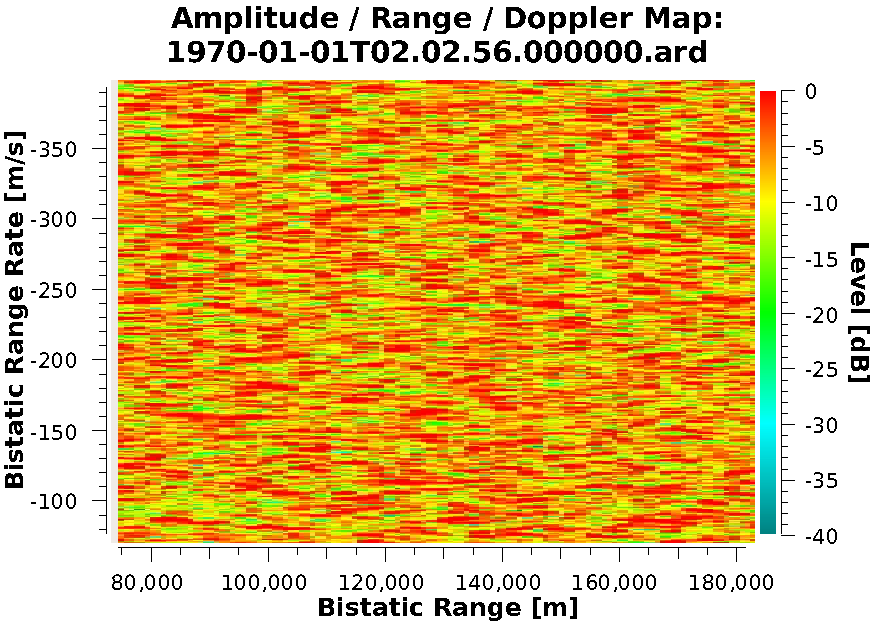
\includegraphics[width=0.7\textwidth]{figs/Simulations/10WJammingPerfectRefARDLast.pdf}
\caption[ARD end of trajectory 10~W jammer.]{ARD at the end of the flight trajectory when 10~W jamming is present in the surveillance channel and no jamming is present in the reference channel.}
\label{fig:10WJammingPerfectRefARDLast}
\end{center}
\end{figure}

\begin{figure}[htbp]
\begin{center}
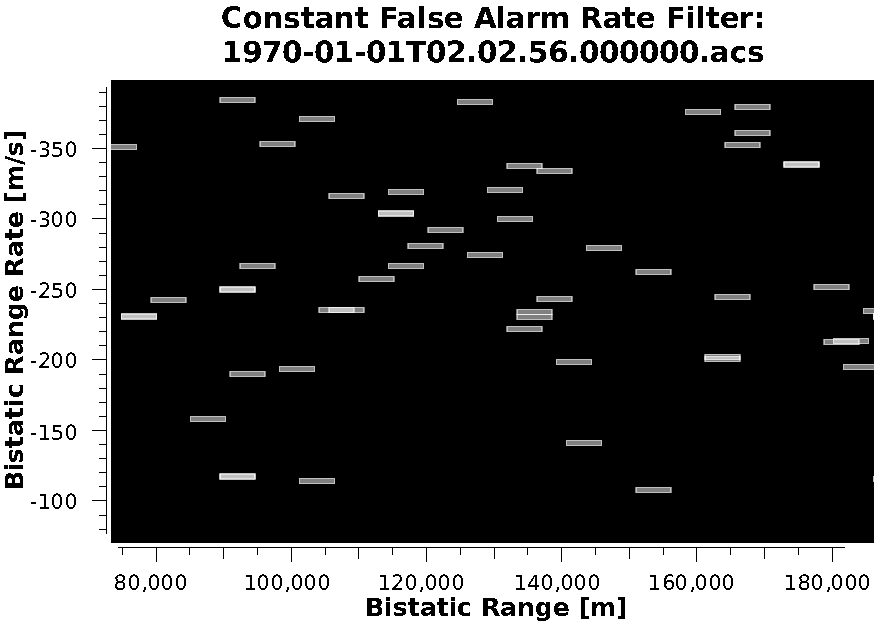
\includegraphics[width=0.7\textwidth]{figs/Simulations/10WJammingPerfectRefCFAR.pdf}
\caption{CFAR history for the duration of the flight trajectory when 10~W jamming is present.}
\label{fig:10WJammingPerfectRefCFAR}
\end{center}
\end{figure}

Inspecting the ARD maps in Figures~\ref{fig:10WJammingPerfectRefARDFirst} and~\ref{fig:10WJammingPerfectRefARDLast}, there is absolutely no visible indication of target position. This is to be expected based on the noise level of the cross-ambiguity function between the FM and jamming signals in Figure~\ref{fig:FMJamCAF}

Observing the CFAR history for a perfect reference in Figure~\ref{fig:10WJammingPerfectRefCFAR} when compared to the case in Figure~\ref{fig:10WJammingCFAR} where there is jamming present in both channels it would appear that the clean reference does in fact produces a lesser SINR based on the detections. This is however speculative and a great deal of statical investigation is necessary to draw a sound conclusion.

\clearpage

\section{Jamming Detection}

The most important part of ECCM is the recognition that the CR system is the victim of ECM of some sort. Here we discuss some techniques that can be used to trigger ECCM i.e the CR must determine that it is a victim.

The jammer might operate in spot or barrage mode. Willis~\cite{willis:07}  discusses the problem that a jammer has in deciding which spot frequency to utilise, especially in the case of FM radio based CR. For the case of single frequency DVB networks, DAB, etc. this is less problematic. Only when the jammer's ESM indicates that only a few FM channels are in operation can the jammer decide to radiate only at one or more spot frequencies. However, only a sophisticated jammer can produce a small number of spot frequencies, and thus the jammer would default to barrage mode.

The CR needs a good ESM system to search for jamming, as will be discussed next.

\subsection{Monitor Transmitter of Opportunity}

All the receivers of the CR system should make intelligent demodulation of the Transmitter of Opportunity. If the normal demodulated signal disappears, it should be a sign of jamming. For example, disappearance of speech or music from the output of an FM demodulation of an FM station being utilised by the CR.

\subsection {Changes in clutter profile}

Since a CR system by definition has no control over the transmitter, it cannot carry out a receiver noise check when the transmitter is off. However, during normal operation, the clutter background dominates, and will be largely constant (zero Doppler). Dramatic changes in this profile can be an indication of strong jamming. The signal levels in the reference or surveillance channel will also be an indicator that there is potential jamming.

\subsection{Other Ideas?}

\todo{Can one see abnormal changes to the clutter background i.e. before cancellation? The CR operates for a long time before being victim, so there will be good statistics.}

If a CR has been operating unimpeded by jamming for a period of time, then a background clutter profile will be known and available. Any deviation and change to the background profile (ultimately varying the statistical performance of the radar) could be an indication of attempted jamming.   


\section{Null Steering}\label{sec:nullsteer}

Depending on the type of CR system, it should be possible to have an array type antenna, and then to have the antenna steer a null towards the jamming source (assuming such a source's position or bearing is known). As shown in Willis~\cite{willis:07}, substantial improvement to CR system performance is possible, at the expense of having a \emph{wedge} taken out of the coverage by the surveillance channel. A conventional ESM with AoA capability would be very useful to find the bearing and presence of a jamming source.

This is illustrated by simulation. Figures~\ref{fig:10WJammingNullSteeringARDFirst},~\ref{fig:10WJammingNullSteeringARDLast} and~\ref{fig:10WJammingNullSteeringCFAR} show results repeating the 10~W jammer scenario described in Section~\ref{sec:Jam10W}. All details are the same except that the surveillance antenna is rotated to the North such that a 7.5 dB null (relative to the 7.2 dBi main lobe) is steered towards the jammer. It is shown that the null provides suitable isolation to allow for target detection. Again the plots have been normalised to the target level which is now slightly lower due the main beam of the surveillance antenna not being centred on the target for the duration of its flight path. While the target is not present in the initial ARD map Figure~\ref{fig:10WJammingNullSteeringARDFirst}, it soon becomes detectable as can be seen by the CFAR history in Figure~\ref{fig:10WJammingNullSteeringCFAR}. The SINR is then clearly discernible by the end of the trajectory as shown in the final ARD map in Figure~\ref{fig:10WJammingNullSteeringARDLast}.

This example uses manual rotation of a fixed beam antenna but this problem would lend itself to digital beam steering provided sufficient dynamic range can be attained.

\begin{figure}[htbp]
\begin{center}
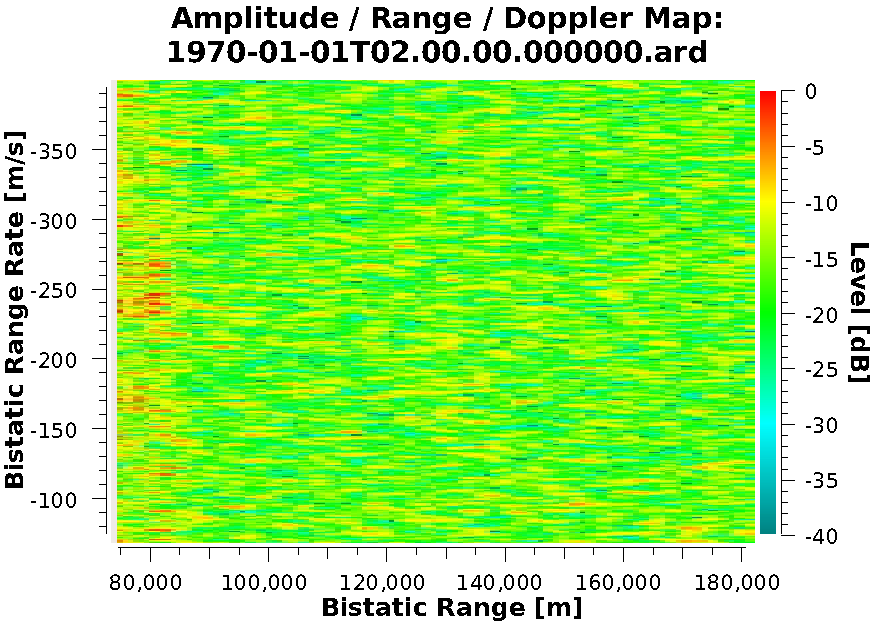
\includegraphics[width=0.7\textwidth]{figs/Simulations/10WJammingNullSteeringARDFirst.pdf}
\caption[ARD with modest null towards jammer.]{ARD at the beginning of the flight trajectory when 10~W jamming is present and a 7.5 dB null relative to boresight gain is steered towards the jammer.}
\label{fig:10WJammingNullSteeringARDFirst}
\end{center}
\end{figure}

\begin{figure}[htbp]
\begin{center}
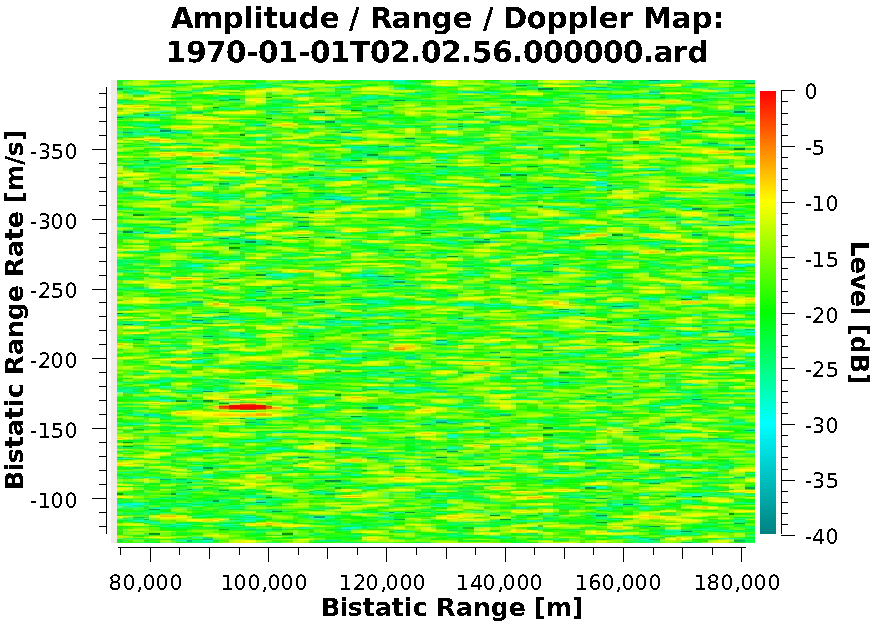
\includegraphics[width=0.7\textwidth]{figs/Simulations/10WJammingNullSteeringARDLast.pdf}
\caption[10~W jammer with null steered.]{ARD at the end of the flight trajectory when 10~W jamming is present and a 7.5 dB null relative to boresight gain is steered towards the jammer.}
\label{fig:10WJammingNullSteeringARDLast}
\end{center}
\end{figure}

\begin{figure}[htbp]
\begin{center}
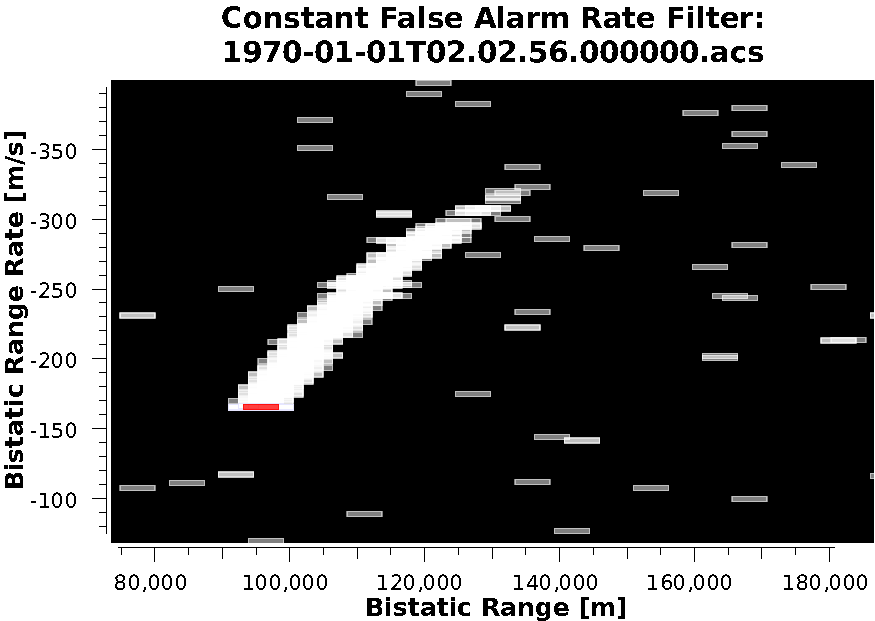
\includegraphics[width=0.7\textwidth]{figs/Simulations/10WJammingNullSteeringCFAR.pdf}
\caption[CFAR history with null steered to jammer of 10~W.]{CFAR history for the duration of the flight trajectory when 10~W jamming is present and a 7.5 dB null relative to boresight gain is steered towards the jammer.}
\label{fig:10WJammingNullSteeringCFAR}
\end{center}
\end{figure}

\clearpage

CR systems that rely on a single receive station, and multiple transmitters will suffer most in terms of loss of angle coverage in utilising this sort of ECCM. However, a CR that uses multiple receive stations, spatially distributed, will have much more flexibility. \todo{A recommendation - \cite{edrich1}} This is somewhat difficult to quantify, as it is so specific to the actual installation of the CR. Arguing loosely, the wedge taken out from each system will point in a different direction, yielding a satisfactory aggregate performance of the system. 

\section{Diversity: Multiple Receivers / Transmitters}

To be able to track targets in two or three dimensions, a CR must employ more than one transmitter or receiver. This is also a requirement of reducing ``ghost'' targets. We have discussed the potential advantages of a spatially diverse system in the previous section, and point out that diversity in terms of either multiple transmitters or receivers is needed for good tracking performance (especially accuracy).

The ECM attacker needs an enormous amount of information, beyond what ESM will yield to be able to set on a reasonable amount of power to all receivers of an ESM system. In fact, depending on the scenario, many of the receivers might even be pointing away from the jammer.

\section{Cancellation of Jamming}

Zheng et al.~\cite{zheng:08} claim more than 20~dB cancellation for a two stage structure, working against inadvertent jamming. This should be investigated further in the light of the ineffectiveness of noise jamming shown in the simulations above.

It seems, based on the simulations, that removal of the jamming from the reference signal (which we did artificially) does not assist dramatically with improvement of the ARD output after CFAR. However, this needs further investigation. As an aside, it seems that a clean reference is very important i.e. it should be free of multipath.




%_________________________________
\section{Recognition of wrong targets}

Due to the variety of deception and CR architecture, one can only mention a few options. As indicated in section~\ref{sec:decoy}, a drone aircraft could be fitted with a transponder. It could then rely on its motion doppler to present one (or, with a multchannel DRFM) or more targets. The speed of the drone will be low and cause suspicion, but a more expensive, jet drone could be used to emulate a fighter attack. In the case of the slow target, the CR would expect this to be a smaller, propeller driven aircraft. In this case, the lack of propeller modulation would be an indication of a false target.

The decoy would, of course, have to have access to the transmitter of opportunity, and if this is unknown, it would need to carry out the deception for all transmitters in sight, which makes the ECM too expensive.


%_________________________________
\section{Sector blanking}

This is a technique used in monostatic radar, in not applicable to the CR. Its analogue is null steering, which is covered in section~\ref{sec:nullsteer}.


%_________________________________
\section{Chaff}
Deployment of chaff is going to be difficult against the majority of CR, since they work at low frequencies, and making the chaff elements long enough to resonate, and, to deploy properly, is going to be very difficult. Calculating the effectiveness of a chaff cloud can proceed in the normal way, except the geometry must be taken into account. Again, a multi-receiver CR is going to make the position for deployment of the cloud to provide sufficient screening a challenge.

The chaff cloud is also not moving, so it will be cancelled by the CR processor, leaving only the effect of attenuation of the CR signal through the chaff cloud to contend with. Clearly, if the cloud is substantial, then the degradation of SNR of targets, and hence, detection will be significant.

%_________________________________
\section{Decoys}\label{sec:decoy}

This is a potentially useful approach, and is depended on DRFM~\ref{sec:drfm}. The technological issues are discussed there. The question is about the effectiveness of a interfering transmitter that emits the original broadcast signals with time delays and / or Doppler shifts, known as repeater techniques (DRFM jamming).

%_________________________________
\section{Deception Waveforms (DRFM)} \label{sec:drfm}
%_________________________________
The success of decoy~\ref{sec:decoy} operations will depend on what waveforms are possible with the DRFM. For FM Band CR, the signal bandwidths are low (100~kHz maximum), making the DRFM device relatively simple. This is not true for DVB and other high bandwidth waveforms. However, the DRFM  system has to cater for a wide range of potential carrier frequencies, which would push up the cost. Further, the system might be required to provide range delay and Doppler shift in order to create false targets.

\section{ECCM Conclusions}

This chapter has reviewed a number of aspects of the ECCM situation. It seems that null steering towards the jamming is an excellent countermeasure to ECM. However, knowing the azimuth angle of the jamming source is clearly important. This points to excellent ESM being required for the CR system. It must be aware of changes in the EM environment in its band of operation. 

Given that an azimuth angle will be needed of adaptive countermeasures, the ESM system must provide the bearing to the jammer signal. As pointed out in the chapter, jamming detection is not necessarily straight forward. However, since the jammer operator is going to be conservative in terms of using higher power, and that the ESM only has a one way propagation path to contend with, it should be possible to use a direction finder to locate the jammer.

The loss of coverage due to jamming is best counteracted by using a multiple receiver architecture. All receivers would be steering a null towards the jammer, and due to the spatial diversity, the system as a whole will not loose coverage, since the relative nulls would not overlap.

Drone technology could provide complex, decoy targets. The CR system would need to have a powerful tracking processor to instantiate tracks and reject the increase in decoy targets. The same would apply for a deception system. 

Low-cost drones with simple beacons would potentially be effective against FM Band CR. However, their slow speed could expose them. Again, a CR multi-receiver architecture makes it almost impossible for the jammer / DRFM to provide a consistent target i.e. with the correct range and Doppler profile for all receivers.




\todo{Daniel, anything to add, after reviewing the simulations etc. above. - I have added in at the specific points so nothing else need be inserted here.}

%================================
\chapter{Conclusions}

The report concludes with a summary of major conclusions, with an indication of where further work is required. As mentioned earlier in this section, this report is scoped to present the possibilities for defeating CR systems, rather than providing detailed analysis of all cases. The possibilities are huge, due to the diverse nature of CR systems, compounded with the geometries.

We first report back directly on the user requirement spelled out in Appendix~\ref{app:urs}, followed by other conclusions arising from the investigation.

\section{Review of User Requirement}
\paragraph{As general overview}

\begin{itemize}

\item \emph{a summary of what is published on EW (probably as well as Cyber Defense topics) on passive radars (probably speculations about activities not publicly published (NATO Group activities, etc.)}
\item There is virtually nothing published in the open literature, except for handwaving statements by most that CR will be robust against ECM.
\item There is an analysis purely in terms of SNR degradation of a bistatic CR, offered in Willis' book~\cite{willis:07}, as well as a general discussion of ECM and ECCM topics.
\item Willis~\cite{willis:07} dispels the myth that a CR system might use the jammer as a source of opportunity: the signal level is too low.
\item There are a number of Chinese papers on CR, but no translations are available. One paper mentions a two stage canceller for inadvertent interference that is worth further investigation.


\item \emph{what are the EW concepts against passive radars and what trends there might be (ECM, ECCM)} 
\item There does not seem to be a coherent, open, discussion of ECM and ECCM with CR.
\end{itemize}
\todo{Is this true? Daniel, anything to add here? - I believe this is true - at least until our paper is published.}

In answer to the last question,

\paragraph{jamming:}


\begin{itemize}
\item\emph{ how is the effectiveness of common jamming methods to disturb passive radars, under the assumption that receiver sites are known / unknown? If possible distinction of cases for single frequency networks (e.g. DAB, DVB) and FM.}
\begin{itemize}
\item  If the sites are known, and a jammer can be sited to provide even reasonable levels of jamming power, it would seem that the CR is very vulnerable. Cancellation techniques seem unlikely, since if they work at high fidelity, they will also remove the signal.
\item If the CR can deploy a special receiver to isolate the jamming signal, an investigation of jammer cancellation in surveillance and if necessary, reference channel should be made.
\item If the receiver sites are unknown, it will be very difficult for the ECM operator to ensure that sufficient jammer power is provided to all the receiver sites, especially since some of them will not be facing the jammer.
\end{itemize}
\end{itemize}

\begin{itemize}
\item \emph{which waveforms are appropriate for jamming (broadband, noise, specific waveforms....)}
\begin{itemize}
\item It seems that any signal that fills the CR's bandwidth will be successful in jamming. 
\end{itemize}
\end{itemize}

\begin{itemize}
\item \emph{power and bandwidth considerations for jamming emitters}
\begin{itemize}
\item Our simulations show that modest amounts of jammer power will severely disturb a CR, in the case that both the reference and the surveillance channel are corrupted. Willis~\cite{willis:05, willis:07} also provides analysis for the simple noise jammer decreasing the SNR.
\item Spot jamming (just the bandwidth in question) will provide the most destructive energy to the channel, whereas a broad bandwidth signal (barrage jamming) will have a reduced effectiveness since the jammer total power is a restriction.
\end{itemize}
\end{itemize}

\begin{itemize}
\item \emph{broadband (noise) jamming}
\begin{itemize}
\item  We have covered this topic in the previous two bullet items above.
\end{itemize}
\end{itemize}

\paragraph{deception:}


\begin{itemize}
\item \emph{indication of wrong targets or wrong target positions. Might be difficult concerning the multistatic geometry (multiple angle illumination of targets)?}
\begin{itemize}
\item As pointed out, the deception jammer will need to have, (a) accurate knowledge of CR geometry, and access to a clean copy of the transmitter of opportunity's transmissions. The jammer would also need to have DRFM capability with variable range pull off / simulation (see next question) and Doppler modulation. This becomes an expensive, highly specialised piece of equipment.
\item A CR system not using AoA techniques could then be deceived, but the complexity of this task is going to rely on a complex and expensive jammer. An AoA based system, similar to monopulse systems, will not be deceived.
\end{itemize}


\item \emph{effectiveness of interfering transmitter which emit the original broadcast signals with time delays and / or Doppler shifts (repeater techniques, DRFM jamming)}
\begin{itemize}
\item  This is an extension of the previous question in that a DRFM with range adjustment could be required for generating a deception target.
\item As stated in the previous question, Doppler simulation would also be needed as none of the moving targets are removed by the CR's MTI type processing. The Doppler profile needs to be matched to the CRs geometry, which is not trivial.
\item It might be a better strategy to put the CRs tracker under pressure by generating many, random, Doppler shifted targets, each of which would need to be sifted by the radar data processor, maybe leading to overload.
\end{itemize}



\end{itemize}

\paragraph{protection against jamming / deception:}

This is typically known as ECCM.

\begin{itemize}
\item \emph{techniques which protect passive radars against jamming / interfering transmitters (recognition of wrong targets or jamming, sector blanking, etc.)}

\begin{itemize}
\item The CR must endeavour to remove all jamming signals that impinge on both reference and surveillance channels, as it is very susceptible to this, and it follows that, 

\begin{itemize}
\item Antenna null steering is the best countermeasure against jamming. This is, of course, at the expense of coverage, and implies that a CR system's antennas must be flexible (capable of null steering).
\item Inherent in the geometry of a multisite (almost all) CR, there is possible redundancy i.e. the jammer may not be effective against all nodes and the system as a whole might still be effective.
\item If the CR system can ensure a clean reference signal, jamming cancellation might be successful. It follows that a multi-receiver CR system will be most successful in this situation, especially if it includes a flexible antenna, capable of null steering.
\item The CR system should have an excellent ESM that can detect and find the bearing angle to the jammers.
\item If a clean version of the jammer signal is available it will provide the best, ghost target free, ARD plot for CFAR.
\end{itemize}
\end{itemize}
\end{itemize}






\paragraph{Converge on Type of CR}


As is clear from this report, the wide range of CR systems available makes it very difficult to provide definitive comments on the best ECM to deploy. To some extent this becomes a, \emph{chicken and egg} situation i.e. one would also wish to choose a CR system that operates best against ECM and would have the best ECCM possibilities.

Given the analysis of noise jamming carried out in Willis~\cite{willis:07}, it would seem that a CR system that operates with a large number of spatially distributed receivers seems best, as this type of system can not only utilise multiple transmitters, but, as a system, can exploit the difficulty the jammer will have to provide directional jamming power to all potential locations.

If the CR system is providing gap filler coverage for isolated values, terrain screening can be an important advantage to the CR system, since the jammer has to operate in specific directions.

\paragraph{Simulation Capability}

It is clear [ref:sims] that for proper tactics to be assessed  against a CR system, proper simulation capability is required. This is especially true if methods other than noise jamming are to be attempted.

%================================
\chapter{Recommendations}

The scope of this report is restricted by the time available, so we list here a number of items that require further investigation.

\begin{enumerate}
\item Military personnel involved in setting up and / or defeating CR systems should receive specialist training to be able to operate with these unconventional radars.
\item There are almost no comprehensive, published, results on the performance of a CR in the presence of most types of jamming. This leads to the next comment i.e.
\item The need for good modelling tools. The large variety of CR type systems possible make it impossible to evaluate all options, and careful studies of the ECM vulnerability and ECCM techniques are necessary. Indeed this is true of planning to defeat such a system (ECM). These activities all require excellent modelling software, coupled with real measurements.
\item It seems that spatial diversity of transmitters and receivers, besides being critical to tracking ability of a CR, also provide good ECCM capabilities.
\item A CR consisting of a number of spatially diverse, networked receivers seems to be the most resilient against ECM and able to mount more ECCM. It is also able to exploit numerous transmitters, making it difficult for all receivers to be taken out in an attack.
\item The position and type of CR system must be kept as secret as possible to keep the attacker uncertain as to which frequencies to jam, and which transmitters to neutralise. Fixed stations should purposely delude spies as to their mode of operation, especially frequency. Dummy antenna systems would be a good decoy.
\item Excellent ESM systems with the capability of detecting jammers (especially noise) and the bearing from the ESM to the jammer. This can be translated for the CR receivers in the system for setting up possible null steering. The ESM system should also be able to locate the jammer due to its spectral shape compared to the normal transmissions of the transmitter of opportunity.
\item Only null steering, and fortuitous gain reduction in the direction of the jammer is effective in improving the performance of a CR in the presence of jamming. The form of the jamming waveform is not important, as long as it occupies a large amount of the band being utilised.
\item A CR system that has access to a clean version of the reference transmitter (which could be base band) could well be able to cancel out the jamming.
\item Forcing the jammer to operate in barrage mode will assist i.e. a multifrequency CR.

\end{enumerate}


%=========== Bibliography =====================
\newpage \addcontentsline{toc}{chapter}{Bibliography} \nocite{*}
\bibliographystyle{vancouver}
\bibliography{commensalED,doh_bib_2}
%================================


%================================
\appendix
%================================
\chapter{User Requirements}\label{app:urs}

The customer has stated these in an email as follows: 

\quote{
Armasuisse is interested in  EW-aspects of passive radars in the context of a superior passive radar project, which has the goal to investigate the performance of passive radar systems and its potential contribution to a sensor network and its recognized air picture. In General, we are interested in passive radar systems which use the common broadcast transceivers and waveforms (FM, DAB, DVB). But we are also open to other systems, e.g. which use their own transceivers emitting  appropriate waveforms which are under control of the operators.}
 
Concerning EW-aspects, the following topics (amongst others) should be covered in the study and are interesting for us:
\begin{itemize}
\item As general overview,


\begin{itemize}
\item a summary of what is published on EW (probably as well as Cyber Defense topics) on passive radars (probably speculations about activities not public published (NATO Group activities, etc.)
\item what are the EW concepts against passive radars and what trends there might be (ECM, ECCM)
\end{itemize}

\item jamming:

\begin{itemize}
\item how is the effectiveness of common jamming methods to disturb passive radars, under the assumption that receiver sites are known / unknown? If possible distinction of cases for single frequency networks (e.g. DAB, DVB) and FM.
\item which waveforms are appropriate for jamming (broadband, noise, specific waveforms....)
\item power and bandwidth considerations for jamming emitters
\item broadband (noise) jamming

\end{itemize}

\item deception:

\begin{itemize}
\item indication of wrong targets or wrong target positions. Might be difficult concerning the multistatic geometry (multiple angle illumination of targets)?
\item effectiveness of interfering transmitter which emit the original broadcast signals with time delays and / or Doppler shifts (repeater techniques, DRFM jamming)
\item protection against jamming / deception:
\item techniques which protect passive radars against jamming / interfering transmitters (recognition of wrong targets or jamming, sector blanking, etc.)
\end{itemize}



\end{itemize}
%=====================================

\label{lastpg}
\end{document}
%=====================================
\begin{figure}
 
\end{figure}

